%--------------------------------------------------------------
% thesis.tex 
%--------------------------------------------------------------
% Corso di Laurea in Informatica 
% http://if.dsi.unifi.it/
% @Facolt\`a di Scienze Matematiche, Fisiche e Naturali
% @Universit\`a degli Studi di Firenze
%--------------------------------------------------------------
% - template for the main file of Informatica@Unifi Thesis 
% - based on Classic Thesis Style Copyright (C) 2008 
%   Andr\'e Miede http://www.miede.de   
%--------------------------------------------------------------
\documentclass[twoside,openright,titlepage,fleqn,
	headinclude,12pt,a4paper,BCOR5mm,footinclude]{scrbook}
%--------------------------------------------------------------
\newcommand{\myItalianTitle}{Raffinamento di una libreria Python per l'OCR di documenti d'identit\`a\xspace}
\newcommand{\myEnglishTitle}{Refinement of a Python library to perform OCR on identity documents\xspace}
\newcommand{\myDegree}{Corso di Laurea in Informatica\xspace}
\newcommand{\myName}{Alessio Falai\xspace}
\newcommand{\myProf}{Maria Cecilia Verri\xspace}
\newcommand{\myOtherProf}{Correlatore\xspace}
\newcommand{\mySupervisor}{Michele Barbagli\xspace}
\newcommand{\myFaculty}{
	Scuola di Scienze Matematiche, Fisiche e Naturali\xspace}
\newcommand{\myUni}{\protect{
	Universit\`a degli Studi di Firenze}\xspace}
\newcommand{\myLocation}{Firenze\xspace}
\newcommand{\myTime}{Anno Accademico 2018-2019\xspace}
\newcommand{\myVersion}{Version 0.1\xspace}
%--------------------------------------------------------------
\usepackage[italian]{babel}
\usepackage[latin1]{inputenc} 
\usepackage[T1]{fontenc}
\usepackage[square,numbers,sort&compress]{natbib}
\usepackage[fleqn]{amsmath}  
\usepackage{ellipsis}
\usepackage{listings}
\usepackage[font=small]{subfig}
\usepackage{caption}
\usepackage{appendix}
\usepackage{siunitx}
\usepackage{nameref}
\usepackage{wrapfig}
\usepackage{tocstyle}
\usetocstyle{allwithdot}
\usepackage{algorithm}
\usepackage[noend]{algpseudocode}
\makeatletter
\renewcommand{\ALG@name}{Algoritmo}
\renewcommand{\listalgorithmname}{Elenco degli algoritmi}
\makeatother
\newcommand{\vars}{\texttt}
\newcommand{\func}{\textrm}
\let\oldReturn\Return
\renewcommand{\Return}{\State\oldReturn}
\captionsetup[subfigure]{format=plain,labelformat=parens,labelsep=newline}
\captionsetup[subfloat]{singlelinecheck=off,justification=centering}
\captionsetup[table]{position=bottom}
\interfootnotelinepenalty=10000
%--------------------------------------------------------------
\usepackage{dia-classicthesis-ldpkg}
%--------------------------------------------------------------
% Options for classicthesis.sty:
% tocaligned eulerchapternumbers drafting linedheaders 
% listsseparated subfig nochapters beramono eulermath parts 
% minionpro pdfspacing
\usepackage[eulerchapternumbers,linedheaders,subfig,beramono,eulermath,
parts]{classicthesis}
%--------------------------------------------------------------
\newlength{\abcd} % for ab..z string length calculation
% how all the floats will be aligned
\newcommand{\myfloatalign}{\centering} 
\setlength{\extrarowheight}{3pt} % increase table row height
\captionsetup{format=hang,font=small}
\setcounter{topnumber}{2}
\setcounter{totalnumber}{1}
\setlength{\skip\footins}{1.3pc plus 5pt minus 2pt}
%--------------------------------------------------------------
% Layout setting
%--------------------------------------------------------------
\usepackage{geometry}
\geometry{
	a4paper,
	ignoremp,
	textwidth     = 13.5cm,
	textheight    = 21.5cm,
	lmargin       = 3.5cm, % left margin
	tmargin       = 4cm    % top margin 
}

\lstset{
  	frame=tb,
	language=Matlab,
  	aboveskip=3mm,
  	belowskip=3mm,
  	showstringspaces=false,
  	columns=flexible,
  	basicstyle={\small\ttfamily},
  	numbers=none,
  	breaklines=true,
  	breakatwhitespace=true,
  	tabsize=3
}
\usepackage{tikz}
\usepackage{pgf}
\usepackage{pgfplots}
\usepackage{mathrsfs}
\usetikzlibrary{arrows}
\usetikzlibrary{backgrounds}
\widowpenalty10000
\clubpenalty10000
%--------------------------------------------------------------
\begin{document}
\frenchspacing
\raggedbottom
\pagenumbering{roman}
\pagestyle{plain}
%--------------------------------------------------------------
% Frontmatter
%--------------------------------------------------------------
%--------------------------------------------------------------
% title.tex (use thesis.tex as main file)
%--------------------------------------------------------------
\begin{titlepage}
	\begin{center}
   	\large
      \hfill
      \vfill
      \begingroup
         
\includegraphics[scale=0.15]{logo/logo-unifi}\\
%			\spacedallcaps{\myUni} \\ 
			\myFaculty \\
			\myDegree \\ 
			\vspace{0.5cm}
         \vspace{0.5cm}    
         Tesi di Laurea    
      \endgroup 
      \vfill 
      \begingroup
      	\color{Maroon}\spacedallcaps{\myItalianTitle} \\ $\ $\\
      	\spacedallcaps{\myEnglishTitle} \\ 	
	\bigskip
      \endgroup
      \spacedlowsmallcaps{\myName}
      \vfill 
      \vfill
      Relatore: \emph\myProf\\
      \vfill
      \vfill
      \myTime
      \vfill                      
	\end{center}        
\end{titlepage}   
%--------------------------------------------------------------
% back titlepage
%--------------------------------------------------------------
   \newpage
	\thispagestyle{empty}
	\hfill
	\vfill
	\noindent\myName: 
	\textit{\myItalianTitle,} 
	\myDegree, \textcopyright\ \myTime
%--------------------------------------------------------------
% back titlepage end
%--------------------------------------------------------------

\pagestyle{scrheadings}
%--------------------------------------------------------------
% Mainmatter
%--------------------------------------------------------------
\pagenumbering{arabic}
% use \cleardoublepage here to avoid problems with pdfbookmark
%\chapter*{Introduzione}
\addcontentsline{toc}{chapter}{Introduzione}
\markboth{Introduzione}{Introduzione}

Questa tesi vuole essere un riassunto delle attivit\`a svolte in un tirocinio curriculare presso l'azienda QI-LAB di Firenze nel periodo \textit{marzo - giugno 2019}. L'offerta di tirocinio prevedeva l'apporto di migliorie, in termini di accuratezza ed efficienza, riguardanti una libreria per il riconoscimento ottico dei caratteri di alcuni campi di documenti d'identit\`a, attualmente solo italiani. La libreria, denominata QI-OCR, era inizialmente il risultato del lavoro compiuto da un precedente tirocinante, \textit{Emilio Cecchini}, che si era occupato dell'implementazione del framework di base, sul quale ho avuto il piacere di lavorare io stesso. QI-OCR viene distribuita come pacchetto \textit{pip} ed \`e stata scritta con linguaggio Python, in versione \textit{3.6.8}, anche se compatibile con la versione minor successiva, ovvero la \textit{3.7.x}, nonch\`e l'ultima versione stabile rilasciata, nella data in cui mi trovo a scrivere questo testo. QI-OCR prevedeva la suddivisione in 4 moduli principali:
\begin{enumerate}
	\item \textbf{Preprocessing}: Si occupa della localizzazione del documento all'interno dell'immagine, del ritaglio dei contorni e del raddrizzamento, tramite l'algoritmo di feature matching \textit{SIFT}.
	\item \textbf{Docfields}: Si occupa di effettuare un ritaglio statico, mediante coordinate predeterminate, dei campi d'interesse del documento gi\`a centrato.
	\item \textbf{OCR}: Si occupa di effettuare una binarizzazione dei campi dell'immagine mediante un algoritmo di sogliatura globale \textit{ad-hoc} e di fornire le immagini prodotte in input a un motore di OCR.
	\item \textbf{Postprocessing}: Si occupa di applicare tecniche di analisi sintattica e semantica sui risultati ritornati dal software OCR.
\end{enumerate}
Il lavoro da me svolto riguarda il miglioramento della libreria QI-OCR, mediante tecniche che verranno descritte successivamente. A tal proposito, la tesi \`e suddivisa in cinque capitoli. Il capitolo \ref{chap:math-prerequisites} presenta una descrizione dei prerequisiti matematici necessari a comprendere correttamente le spiegazioni dei metodi presenti nei capitoli successivi. Il capitolo \ref{chap:image-binarization} riguarda lo studio e l'implementazione di tecniche di binarizzazione e segmentazione di immagini, ovvero soluzioni necessarie per la "pulizia" di una generica immagine contenente testo, che permettano di ottenere idealmente il solo testo di colore nero e tutto il resto di colore bianco. Il capitolo \ref{chap:image-matching} riguarda invece lo studio di algoritmi di segmentazione basata dal riscontro sul modello, in cui vengono introdotti metodi alternativi al ben noto SIFT per l'individuazione della posizione di un documento all'interno di un'immagine. Il capitolo \ref{chap:text-detection} introduce l'applicazione di tecniche avanzate di \textit{text-detection} con lo scopo di colmare problemi derivanti da documenti che non rispettano alcun tipo di template prefissato, come ad esempio la vecchia carta d'identit\`a cartacea italiana, che risulta comunque rilasciabile, in alternativa alla nuova carta d'identit\`a elettronica italiana, in casi di estrema esigenza o per tutti i cittadini che non possono recarsi per motivi di handicap presso il municipio. Infine, il capitolo \ref{chap:improvements} descrive ulteriori migliorie e innovazioni introdotte, sia per quanto riguarda il lato sviluppo/distribuzione (containerizzazione, benchmarks, \dots), sia per quanto riguarda l'esperienza utente (OCR parametrizzabile sui campi del documento, implementazione di diversi motori di OCR, \dots).
 % use \myChapter command instead of \chapter
\setcounter{tocdepth}{1}
\tableofcontents
\addtocontents{lof}{\protect\enlargethispage{\baselineskip}}
\listoffigures
\cleardoublepage
\thispagestyle{empty}
\begin{flushright}
\null\vspace{\stretch {1}}
\emph{"If a machine is expected to be infallible, it cannot also be intelligent" \break --- Alan Turing} \vspace{\stretch{2}}\null
\end{flushright}
\cleardoublepage
\chapter*{Introduzione}
\addcontentsline{toc}{chapter}{Introduzione}
\markboth{Introduzione}{Introduzione}

Questa tesi vuole essere un riassunto delle attivit\`a svolte in un tirocinio curriculare presso l'azienda QI-LAB di Firenze nel periodo \textit{marzo - giugno 2019}. L'offerta di tirocinio prevedeva l'apporto di migliorie, in termini di accuratezza ed efficienza, riguardanti una libreria per il riconoscimento ottico dei caratteri di alcuni campi di documenti d'identit\`a, attualmente solo italiani. La libreria, denominata QI-OCR, era inizialmente il risultato del lavoro compiuto da un precedente tirocinante, \textit{Emilio Cecchini}, che si era occupato dell'implementazione del framework di base, sul quale ho avuto il piacere di lavorare io stesso. QI-OCR viene distribuita come pacchetto \textit{pip} ed \`e stata scritta con linguaggio Python, in versione \textit{3.6.8}, anche se compatibile con la versione minor successiva, ovvero la \textit{3.7.x}, nonch\`e l'ultima versione stabile rilasciata, nella data in cui mi trovo a scrivere questo testo. QI-OCR prevedeva la suddivisione in 4 moduli principali:
\begin{enumerate}
	\item \textbf{Preprocessing}: Si occupa della localizzazione del documento all'interno dell'immagine, del ritaglio dei contorni e del raddrizzamento, tramite l'algoritmo di feature matching \textit{SIFT}.
	\item \textbf{Docfields}: Si occupa di effettuare un ritaglio statico, mediante coordinate predeterminate, dei campi d'interesse del documento gi\`a centrato.
	\item \textbf{OCR}: Si occupa di effettuare una binarizzazione dei campi dell'immagine mediante un algoritmo di sogliatura globale \textit{ad-hoc} e di fornire le immagini prodotte in input a un motore di OCR.
	\item \textbf{Postprocessing}: Si occupa di applicare tecniche di analisi sintattica e semantica sui risultati ritornati dal software OCR.
\end{enumerate}
Il lavoro da me svolto riguarda il miglioramento della libreria QI-OCR, mediante tecniche che verranno descritte successivamente. A tal proposito, la tesi \`e suddivisa in cinque capitoli. Il capitolo \ref{chap:math-prerequisites} presenta una descrizione dei prerequisiti matematici necessari a comprendere correttamente le spiegazioni dei metodi presenti nei capitoli successivi. Il capitolo \ref{chap:image-binarization} riguarda lo studio e l'implementazione di tecniche di binarizzazione e segmentazione di immagini, ovvero soluzioni necessarie per la "pulizia" di una generica immagine contenente testo, che permettano di ottenere idealmente il solo testo di colore nero e tutto il resto di colore bianco. Il capitolo \ref{chap:image-matching} riguarda invece lo studio di algoritmi di segmentazione basata dal riscontro sul modello, in cui vengono introdotti metodi alternativi al ben noto SIFT per l'individuazione della posizione di un documento all'interno di un'immagine. Il capitolo \ref{chap:text-detection} introduce l'applicazione di tecniche avanzate di \textit{text-detection} con lo scopo di colmare problemi derivanti da documenti che non rispettano alcun tipo di template prefissato, come ad esempio la vecchia carta d'identit\`a cartacea italiana, che risulta comunque rilasciabile, in alternativa alla nuova carta d'identit\`a elettronica italiana, in casi di estrema esigenza o per tutti i cittadini che non possono recarsi per motivi di handicap presso il municipio. Infine, il capitolo \ref{chap:improvements} descrive ulteriori migliorie e innovazioni introdotte, sia per quanto riguarda il lato sviluppo/distribuzione (containerizzazione, benchmarks, \dots), sia per quanto riguarda l'esperienza utente (OCR parametrizzabile sui campi del documento, implementazione di diversi motori di OCR, \dots).

\chapter{Alcuni prerequisiti matematici nell'ambito della computer vision}
\label{chap:math-prerequisites}


\section{Immagini digitali}
Un'immagine digitale \textit{I} con risoluzione $m\times n$ \`e una matrice di valori interi di dimensione $n\times m$, che pu\`o essere matematicamente interpretata come una funzione semplice (n\`e iniettiva n\`e suriettiva) \textit{I}: $\mathbb{N}\times\mathbb{N}\supseteq X \to \mathbb{P}^{c}$, che si occupa di mappare una coppia ordinata $(u,v)\in\mathbb{N}\times\mathbb{N}$, con $u,v\in\mathbb{N}$, in una \textit{c-upla} $p=(p_{1}, p_{2}, \dots, p_{c})$, in cui ciascun valore $p_{i}$ di $p$ rappresenta il valore del pixel associato nel canale ${i}$, con $0 \leq p_{i} \leq 2^{b} - 1$, dove $b$ \`e il numero fissato di bit utilizzati per rappresentare ciascun pixel e $2^{b}$ indica il massimo numero di colori o di livelli di grigio utilizzabili. Per esempio, ipotizzando di utilizzare canali colore standard, nel caso in cui si lavori con immagini in scala di grigi si avr\`a $c=1$, mentre nel caso in cui si lavori con immagini \textit{RGB} si avr\`a $c=3$ ($c=4$ per immagini \textit{RGBA} o \textit{CMYK}). Inoltre, supponendo di utilizzare una profondit\`a pari a $b=8$ sar\`a possibile specificare interi compresi tra $0$ e $255$ per i valori di ciascun pixel. Infine, indichiamo la risoluzione dell'immagine come la coppia $(m, n)\in\mathbb{N}\times\mathbb{N}\colon(n, m)=\max_{(x, y)\in X} (x,y)$.


\section{Convoluzione}
La \textit{convoluzione} \`e un'operazione alla base dell'\textit{image processing}, grazie alla quale \`e possibile andare ad analizzare ed eventualmente accentuare o alleviare diversi aspetti di una data immagine, come la sfocatura, la nitidezza, i contorni e molto altro. L'operazione, che viene descritta nella forma discreta, prende dunque in input due immagini digitali, ovvero l'immagine originale \textit{I} (normalmente un singolo canale) e l'immagine $K$, denominata \textit{kernel}, e intuitivamente si occupa di far scorrere la matrice $K$ sull'immagine $I$, generalmente a partire dal bordo in alto a sinistra, effettuando una somma pesata dei valori di $I$ dati dalle proiezioni delle posizioni correntemente analizzate dalla matrice $K$, in cui i pesi sono dati proprio dagli elementi di $K$. Solitamente la dimensione della matrice $K$ \`e molto minore della dimensione dell'immagine originale e spesso $K$ \`e una matrice quadrata $n\times n$, con $n$ dispari. Pi\`u formalmente, l'operazione di \textit{convoluzione} $I * K$ in un punto $(i,j)$ \`e data da:
\begin{equation}
	\label{eq:convolution}
	\begin{split}
		I^{*}(i, j) & = \sum_{x = -n}^{n}\sum_{y = -n}^{n}(I(i-x, j-y)\cdot K(x,y))=\\
		& = \sum_{x = 1}^{n}\sum_{y = 1}^{n}(I(i + \left\lceil{\dfrac{n}{2}}\right\rceil - x, j + \left\lceil{\dfrac{n}{2}}\right\rceil - y)\cdot K(x,y))
	\end{split}
\end{equation}
Nel caso in cui nella formula \ref{eq:convolution} i segni \textit{-} e \textit{+} venissero invertiti si otterrebbe la formulazione della \textit{correlazione} $I \otimes K$ in un punto $(i,j)$:
\begin{equation}
	\label{eq:correlation}
	\begin{split}
		I^{\otimes}(i, j) & = \sum_{x = -n}^{n}\sum_{y = -n}^{n}(I(i+x, j+y)\cdot K(x,y))=\\
		& = \sum_{x = 1}^{n}\sum_{y = 1}^{n}(I(i - \left\lceil{\dfrac{n}{2}}\right\rceil + x, j - \left\lceil{\dfrac{n}{2}}\right\rceil + y)\cdot K(x,y))
	\end{split}
\end{equation}
\textit{Convoluzione} e \textit{correlazione} possono risultare equivalenti se per passare da un'operazione all'altra si effettua un ribaltamento orizzontale e verticale del filtro (graficamente $K$ viene ruotata di $180^{\circ}$). Dunque le due operazioni risultano identiche nel caso in cui la matrice $K$ sia simmetrica rispetto ai due assi. In particolare, si preferisce utilizzare la convoluzione quando sono necessarie le propriet\`a commutativa, associativa e distributiva. Inoltre, dato che spesso il risultato delle operazioni descritte viene utilizzato come valore di intensit\`a di pixel, tale risultato viene normalizzato, dividendolo per la somma dei pesi del filtro. La complessit\`a computazionale delle operazioni, data ad esempio un'immagine di dimensione $m\times m$ e un kernel di dimensione $n\times n$, \`e piuttosto elevata, dato che richiede un numero di moltiplicazioni pari a $n^{2}\cdot m^{2}$ e altrettante somme. Di seguito un esempio di convoluzione e correlazione:
$$
I=\bordermatrix{
		& & & j & & \cr
        & & & \dots & & \cr
		& & 30 & 28 & 32 & \cr
		i & \vdots & 27 & 26 & 10 & \vdots \cr
		& & 29 & 22 & 18 & \cr
		& & & \dots & & \cr
	},
K=\begin{pmatrix} 
	4 & -2 & 1 \\
	-1 & 5 & -3\\
	-6 & 0 & 4
\end{pmatrix}
$$
Calcoliamo $I * K$ nella posizione $(i, j)$ come $$I^{*}(i, j) = 18\cdot 4 - 22\cdot 2 + 29\cdot 1 - 10\cdot 1+ 26\cdot 5 -27\cdot 3 - 32\cdot 6 + 28\cdot 0 + 30\cdot 4 = 24,$$
mentre calcoliamo $I \otimes K$ nella posizione $(i, j)$ come $$I^{\otimes}(i, j) = 30\cdot 4 - 28\cdot 2 + 32\cdot 1 - 27\cdot 1+ 26\cdot 5 -10\cdot 3 - 29\cdot 6 + 22\cdot 0 + 18\cdot 4 = 67$$
Un problema che pu\`o risultare evidente riguarda il modo di trattare i bordi, nel caso in cui l'intorno di un pixel non sia disponibile. Per ovviare a tale problema esistono diverse tecniche valide, come ipotizzare che i pixel non disponibili abbiano intensit\`a zero, oppure prolungare i pixel di bordo supponendo intensit\`a costante in quelli non disponibili.\\
Alcuni esempi di filtri classici:
\begin{itemize}
	\item Sfocatura (filtro di \textit{Gauss}): $\begin{pmatrix} 
		1 & 2 & 1 \\
		2 & 4 & 2\\
		1 & 2 & 1
	\end{pmatrix}$
	\item Nitidezza: $\begin{pmatrix} 
		0 & -1 & 0 \\
		-1 & 5 & -1\\
		0 & -1 & 0
	\end{pmatrix}$
	\item Contorni (filtro di \textit{Laplace}): $\begin{pmatrix} 
		-1 & -1 & -1 \\
		-1 & 8 & -1\\
		-1 & -1 & -1
	\end{pmatrix}$
\end{itemize}


\section{Elementi di morfologia}

\subsection{Basi della matematica morfologica}
La matematica morfologica \`e una collezione di operatori, basata sulla teoria degli insiemi e definita su una struttura astratta\footnote{La struttura astratta alla quale si fa riferimento \`e un \textit{reticolo} infinito, un'estensione della teoria degli insiemi di Minkowski.}. Il suo obiettivo \`e quello di analizzare le forme e gli oggetti di un'immagine digitale, attraverso trasformazioni quali erosione, dilatazione, apertura, chiusura e altre. Nella loro forma originaria le operazioni morfologiche prevedono l'utilizzo di un'\textit{immagine binaria} a singolo canale, composta da pixel che possono assumere solo due valori, 1 e 0, bianco e nero, \textit{foreground} e \textit{background}, oltre che di un \textit{elemento strutturante} (\textit{SE}), anch'esso sotto forma di immagine binaria a singolo canale, generalmente di dimensione molto minore di quella dell'immagine originale. Per correttezza, da ora in poi, in questa sezione, considereremo un'immagine binaria \textit{I} anche come un insieme di punti $Q_{I}$ contenente tutte le coppie $(u,v)$ di pixel \textit{foreground} di \textit{I}, ovvero tali che $I(u, v) = 1$ e considereremo i termini in \textbf{grassetto} come coppie ordinate $(u,v) \in \mathbb{N}\times\mathbb{N}$.
\begin{figure}[t]
	\centering
	\subfloat[Prima (dopo)] {
		\resizebox{6cm}{5cm}{%
		\begin{tikzpicture}[framed,background rectangle/.style={draw=black,fill=black},scale=1.5]
			\draw [fill=white] plot [smooth cycle] coordinates {(0,0) (1,1) (3,1) (1,0) (2,-1)};
		\end{tikzpicture}
		}
	}
	\subfloat[Dopo (prima)] {
		\resizebox{6cm}{5cm}{%
		\begin{tikzpicture}[framed,background rectangle/.style={draw=black,fill=black},scale=1.5]
			\draw [fill=white,scale=0.3] plot [smooth cycle] coordinates {(0,0) (1,1) (3,1) (1,0) (2,-1)};
		\end{tikzpicture}
		}
	}
	\caption{Esempio di erosione (dilatazione) morfologica con elemento strutturante rettangolare} \label{fig:erosion-dilation}
\end{figure}
\par Di seguito una descrizione degli operatori morfologici di base:\\
Il risultato dell'operazione di \textit{erosione} di un'immagine mostra dove lo SE viene contenuto negli oggetti dell'immagine, ovvero, intuitivamente permette di rimuovere pixel dal contorno di \textit{componenti connesse}\footnote{Una \textit{componente connessa} \textit{C} di un insieme di punti \textit{foreground} $P$ di un'immagine binaria $I$ \`e un insieme $C\subseteq P$ tale che $\forall \textbf{p}_{1}, \textbf{p}_{n} \in C$ esiste un percorso $\textbf{p}_{1}, \dots, \textbf{p}_{n}$ in cui ogni $\textbf{p}_{i}$ \`e \textit{k-vicino} (\textit{4-vicino} o \textit{8-vicino}) a $\textbf{p}_{i-1}$ e $\neg \exists \textbf{q}\notin P$ \textit{k-adiacente} a un punto di $P$. \cite{bib:binary-images-connectivity}} di colore bianco, in quantit\`a dipendente dalla grandezza dello SE. In formule:
\begin{equation}
	\label{eq:erosion}
	[\epsilon_{Q_{SE}}(I)](\textbf{x}) = \underset{\textbf{s}\in Q_{SE}}{\bigwedge}(I(\textbf{x}+\textbf{s}))
\end{equation}
Il risultato dell'operazione di \textit{dilatazione} di un'immagine mostra dove lo SE tocca gli oggetti dell'immagine, ovvero, intuitivamente permette di aggiungere pixel al contorno di componenti connesse di colore bianco, in quantit\`a dipendente dalla grandezza dello SE. In formule:
\begin{equation}
	\label{eq:dilation}
	[\delta_{Q_{SE}}(I)](\textbf{x}) = \underset{\textbf{s}\in Q_{SE}}{\bigvee}(I(\textbf{x}+\textbf{s}))
\end{equation}

Le operazioni di \textit{apertura} (\textit{chiusura}) sono invece la combinazione in sequenza di erosione (dilatazione) e dilatazione (erosione) dello SE con la propria \textit{riflessione}\footnote{La \textit{riflessione} di un insieme di punti $P$ di un'immagine binaria $I$ rispetto all'origine viene definita come $\check{P}=\{(-u,-v) \colon (u,v)\in P\}$.}. Queste due operazioni vengono molto utilizzate per rimuovere "sporco" (\textit{noise}) dalle immagini e per "chiudere" piccoli "buchi" all'interno di oggetti che si trovano nel \textit{foreground}. In formule:
\begin{equation}
	\label{eq:opening}
	\gamma_{Q_{SE}}(I) = \delta_{\check{Q_{SE}}}(\epsilon_{Q_{SE}}(I)),
\end{equation}
\begin{equation}
	\label{eq:closing}
	\phi_{Q_{SE}}(I) = \epsilon_{\check{Q_{SE}}}(\delta_{Q_{SE}}(I))
\end{equation}
\par

\begin{figure}[t]
	\centering
	\subfloat[Prima] {
		\begin{tikzpicture}[framed,background rectangle/.style={draw=black,fill=black},scale=0.8]
			\draw [fill=white] plot [smooth cycle] coordinates {(0,0) (1,1) (3,1) (1,0) (2,-1)};
			\draw [fill=white] plot [smooth cycle] coordinates {(4,0) (4,2) (7,0) (5,0) (5,-2)};
			\draw [fill=white] (4,3) circle (0.1cm);
			\draw [fill=white] (3,2) circle (0.2cm);
			\draw [fill=white] (1,-2) circle (0.15cm);
			\draw [fill=white] (7,-2) circle (0.08cm);
		\end{tikzpicture}
	}
	\subfloat[Dopo] {
		\begin{tikzpicture}[framed,background rectangle/.style={draw=black,fill=black},scale=0.8]
			\draw [fill=white] plot [smooth cycle] coordinates {(0,0) (1,1) (3,1) (1,0) (2,-1)};
			\draw [fill=white] plot [smooth cycle] coordinates {(4,0) (4,2) (7,0) (5,0) (5,-2)};
			\draw [fill=black] (4,3) circle (0.1cm);
			\draw [fill=black] (1,-2) circle (0.15cm);
		\end{tikzpicture}
	}
	\caption{Esempio di apertura morfologica con elemento strutturante circolare} \label{fig:opening}
\end{figure}

\subsection{Ricostruzione morfologica}
La \textit{ricostruzione} \`e un'operazione molto utile nella matematica morfologica, che viene spesso presentata come un insieme di operatori \textit{geodetici}, che consentono di estrarre le componenti connesse dell'immagine originale, marcate da un'altra immagine \textit{marker}. Dunque, gli operatori di \textit{erosione} e \textit{dilatazione} possono essere ridefiniti in senso \textit{geodetico}. In particolare, consideriamo al solito un'immagine binaria \textit{I} (\textit{mask}), definita dal suo insieme di punti \textit{foreground} $Q_{I}$, un elemento strutturante (SE), che definisce la connettivit\`a da rispettare, e un'immagine \textit{marker} \textit{F} tale che $Q_{F} \subseteq Q_{I}$, che permette di definire quali componenti connesse devono subire i risultati delle operazioni morfologiche. A questo punto, possiamo definire l'\textit{erosione condizionale} come:
\begin{equation}
	\label{eq:conditional-erosion}
	[\epsilon_{Q_{SE}}(F)]^{(0)}_{I}(\textbf{x}) = [\epsilon_{Q_{SE}}(F)](\textbf{x}) \vee I(\textbf{x})
\end{equation}
e la \textit{dilatazione condizionale} come:
\begin{equation}
	\label{eq:conditional-dilation}
	[\delta_{Q_{SE}}(F)]^{(0)}_{I}(x) = [\delta_{Q_{SE}}(F)](\textbf{x}) \wedge I(\textbf{x})
\end{equation}
Le varianti \textit{geodetiche} vengono definite in modo iterativo a partire da quelle \textit{condizionali}. Dunque, si avr\`a che l'\textit{erosione geodetica} pu\`o essere espressa come:
\begin{equation}
	\label{eq:geodesic-erosion}
	[\epsilon_{Q_{SE}}(F)]^{(i)}_{I}(\textbf{x}) = [\epsilon_{Q_{SE}}([\epsilon_{Q_{SE}}(F)]^{(i-1)}_{I}(\textbf{x}))]^{(0)}_{I}(\textbf{x}), i=1,2,3,\dots,
\end{equation}
mentre la \textit{dilatazione geodetica}:
\begin{equation}
	\label{eq:geodesic-dilation}
	[\delta_{Q_{SE}}(F)]^{(i)}_{I}(\textbf{x}) = [\delta_{Q_{SE}}([\delta_{Q_{SE}}(F)]^{(i-1)}_{I}(\textbf{x}))]^{(0)}_{I}(\textbf{x}), i=1,2,3,\dots
\end{equation}
Concettualmente, le iterazioni sopra definite potrebbero continuare indefinitamente, ma per ragioni pratiche si sceglie di farle terminare per un intero \textit{n} tale che nessun cambiamento avvenga $\forall n' > n$. L'output stabile $R^{\epsilon}_{I}(Q_{F}))=[\epsilon_{Q_{SE}}(F)]^{(n)}_{I}(\textbf{x})$ e $R^{\delta}_{I}(F))=[\delta_{Q_{SE}}(F)]^{(n)}_{I}(\textbf{x})$ cos\`i definito viene denominato rispettivamente \textit{erosione} e \textit{dilatazione} con \textit{ricostruzione}.
\par Definiamo adesso le operazioni di \textit{apertura} e \textit{chiusura} con \textit{ricostruzione}:\\
L'operazione di apertura permette di rimuovere oggetti in base allo SE usato, ma ha il limite di non preservare le altre strutture, che vengono comunque modificate. Questo limite viene completamente superato dall'operatore di \textit{apertura con ricostruzione}, che opera nel seguente modo: l'immagine viene erosa con lo SE come per l'apertura normale, ma invece di far seguire una dilatazione, si opera una ricostruzione usando l'immagine originale come \textit{mask}, e l'immagine erosa come \textit{marker}. L'operazione di \textit{chiusura con ricostruzione} opera in modo analogo. In formule:
\begin{equation}
	\label{eq:opening-reconstruction}
	\tilde{\gamma}_{R}(I) = \gamma_{R}^{(n)}(I) = R_{I}^{\delta}[\epsilon^{(n)}(I)],
\end{equation}
\begin{equation}
	\label{eq:closing-reconstruction}
	\tilde{\phi}_{R}(I) = \phi_{R}^{(n)}(I) = R_{I}^{\epsilon}[\delta^{(n)}(I)]
\end{equation}

\subsection{Altri operatori}
Gli operatori fin'ora descritti permettono di estrarre caratteristiche importanti all'interno delle immagini, ma, ad esempio, consentono difficilemente di effettuare un'equalizzazione di parametri di sfondo, oppure di estrarre piccoli particolari d'interesse, oppure ancora di rilevare i contorni di un oggetto. Per ovviare a queste problematiche, si pu\`o ricorrere all'utilizzo di trasformazioni pi\`u specifiche, derivate da quelle di base. In particolare, possiamo definire l'operatore \textit{top-hat}, nelle due versioni \textit{bianca} e \textit{nera}, rispettivamente:
\begin{equation}
	\label{eq:white-top-hat}
	g_{Q_{SE}}^{w}(I) = I - \gamma_{Q_{SE}}(I),
\end{equation}
\begin{equation}
	\label{eq:black-top-hat}
	g_{Q_{SE}}^{b}(I) = \phi_{Q_{SE}}(I) - I
\end{equation}
Entrambi ritornano un'immagine contenente gli elementi dell'immagine originale che sono pi\`u piccoli dello SE. Il primo ritorna inoltre solo gli elementi pi\`u \textit{luminosi} degli oggetti a loro vicini, mentre il secondo solo gli elementi pi\`u \textit{scuri} degli oggetti a loro vicini. Questo ci fa capire che un buon utilizzo per questo operatore riguarda la correzione di condizioni di luce non uniforme all'interno di un'immagine, per consentire una separazione tra \textit{foreground} e \textit{background} pi\`u marcata, grazie al conseguente incremento di contrasto.
\par Altri operatori morfologici sono quello \textit{hit-or-miss}, che consente di estrarre pixel i cui vicini hanno una specifica configurazione (\textit{pattern}), in base allo SE utilizzato; oppure quello del \textit{gradiente}, che consiste nella differenza tra dilatazione e erosione di un'immagine, e restituisce, ad esempio, i contorni di oggetti.

\chapter{Binarizzazione di immagini}
\label{chap:image-binarization}


\section{Introduzione}
\label{sec:image-bin-intro}
Nel campo dell'\textit{image processing} ricopre un ruolo fondamentale la possibilit\`a di distinguere diversi oggetti, forme e contorni presenti nell'immagine in analisi. Per far ci\`o \`e possibile ricorrere a svariate metodologie, che sono strettamente dipendenti dal contesto in cui si intende operare. Per esempio, nel caso del \textit{riconoscimento ottico dei caratteri} (OCR), le operazioni che andranno descritte assumono importanza assoluta, dato che questo tipo di applicazione, per operare al meglio, ha spesso bisogno di ricevere in input un'immagine in bianco e nero, in cui lo sfondo \`e di colore bianco e il testo \`e di colore nero. Gli argomenti affrontati, nel caso di un'applicazione OCR, saranno soprattutto utili nel caso in cui il motore utilizzato sia \textit{open-source} (vedi \textit{Tesseract}), ovvero nel caso in cui un buon \textit{pre-processing} dell'immagine possa fare la differenza. In questo articolo andremo quindi ad analizzare gli \textit{algoritmi} pi\`u ricorrenti nell'ambito del \textit{thresholding} di immagini e nella sezione \ref{sec:image-bin-proposed-approach} affronteremo un approccio specificamente studiato per i casi d'uso della libreria QI-OCR.

Da qui in avanti ipotizzeremo di lavorare con immagini originali in \textit{scala di grigi} con profondit\`a 8 bit, anche se i metodi descritti possono facilmente essere generalizzati per immagini con pi\`u di un canale colore.


\section{Sogliatura globale}
\label{sec:image-bin-global}
\`E il pi\`u semplice metodo di \textit{thresholding}, che prevede la scelta di un determinato valore di soglia, compreso tra 0 e 255. L'algoritmo di sogliatura prevede quindi la scansione, pixel per pixel, dell'immagine e, nel caso in cui il valore del pixel esaminato sia minore del valore di soglia, tale pixel assumer\`a valore zero, che corrisponde al colore nero. Altrimenti, nel caso in cui il valore del pixel esaminato sia maggiore o uguale del valore di soglia, tale pixel assumer\`a valore 255, che corrisponde al colore bianco. Risulta facile intuire quale possa essere il problema principale di questo tipo di algoritmo di sogliatura, ovvero la scelta del valore di soglia.
Nel caso in cui il contesto in cui si opera sia relativamente statico, la \textit{sogliatura globale} risulta comunque l'opzione pi\`u consigliata, per la sua facilit\`a di implementazione. In particolare, il metodo descritto risulta adatto se le immagini in analisi presentano all'incirca caratteristiche uniformi in termini di illuminazione e contrasto. Se cos\`i non fosse, sarebbe necessario valutare l'implementazione di algoritmi leggermente pi\`u complessi.
\begin{algorithm}
	\caption{Sogliatura globale}
	\label{alg:thresh-global}
	\begin{algorithmic}[1]
		\Function{global-thresholding}{}
			\State $\vars{image} \gets \text{input image}$
			\State $\vars{thresh} \gets \text{threshold value}$
			
			\For {$\vars{i} \text{ in \textproc{rows}(\vars{image})}$}
				\For {$\vars{j} \text{ in \textproc{columns}(\vars{image})}$}
					\If {$\vars{image[i][j]} \geq \vars{thresh}$}
						\State $\vars{image[i][j]} \gets 255$
					\Else
						\State $\vars{image[i][j]} \gets 0$
					\EndIf
				\EndFor
			\EndFor

			\Return $\vars{image}$
		\EndFunction
	\end{algorithmic}
\end{algorithm}


\section{Sogliatura adattativa (o locale)}
\label{sec:image-bin-local}
Questo metodo di \textit{thresholding} consente di sopperire alle mancanze della sogliatura globale, nel caso in cui le immagini in analisi presentino illuminazione e/o contrasto non uniforme. In particolare, questa tecnica dinamica computa automaticamente differenti valori di soglia per diverse aree dell'immagine. Dunque, l'immagine viene suddivisa in tante \textit{sotto-immagini}, abbastanza piccole da poter ipotizzare che in ciascuna illuminazione e contrasto siano sufficientemente uniformi. Una volta partizionata l'immagine, un valore di soglia viene calcolato per ciascuna \textit{finestra}. Il calcolo di ogni valore di soglia dipende dall'implementazione specifica dell'algoritmo, ma genericamente si ricorre all'utilizzo, per ogni sotto-immagine, di semplici operatori statistici, come la media, la mediana o la media fra massimo e minimo.\par
Alcune tecniche di sogliatura locale efficaci sono implementate da algoritmi quali quello di \textit{Niblack} \cite{bib:niblack} e \textit{Sauvola} \cite{bib:sauvola}. In particolare, l'algoritmo di \textit{Niblack} prevede l'utilizzo delle metriche di media e deviazione standard, per una specifica finestra centrata su ciascun pixel dell'immagine. La formula utilizzata per calcolare un generico valore di soglia \`e data da:
\begin{equation}
	\label{eq:niblack}
	T(x, y) = m(x, y) + k \cdot s(x, y),
\end{equation}
dove $T(x, y)$ indica il valore di soglia per il pixel in posizione $(x, y)$, $m(x, y)$ ($s(x, y)$) indica la media (deviazione standard) dei valori dei pixel vicini a quello centrato sulla finestra corrente e $k$ \`e un coefficiente, che pu\`o essere determinato empiricamente\footnote{\textit{Niblack} consiglia l'impostazione del parametro $k$ al valore $-0.2$.}.\par
L'utilizzo di parametri configurabili \`e molto comune per algoritmi di questo tipo, in quanto questi risultano essere fortemente dipendenti dal contesto di utilizzo. Un esempio pratico riguarda la libreria \textit{OpenCV}, che nella funzione $\textproc{adaptiveThreshold}$ consente di selezionare un valore $c$, che viene sottratto da ciascun valore di soglia di ogni sotto-immagine. Per esempio, nel caso in cui il valore di soglia venga calcolato utilizzando la media $mean$, il limite scelto non sar\`a esattamente $mean$, ma $mean - c$.\par
Purtroppo, il problema principale della sogliatura adattativa \`e che tende a valorizzare tutti gli elementi presenti nell'immagine, non consentendo di differenziare al meglio le componenti d'interesse da quelle che invece si vorrebbero scartare.
\begin{algorithm}
	\caption{Sogliatura adattativa}
	\label{alg:thresh-local}
	\begin{algorithmic}[1]
		\Function{local-thresholding}{}
			\State $\vars{image} \gets \text{input image}$
			
			\For {$\vars{pixel} \text{ in \vars{image}}$}
				\State $\vars{thresh} \gets \textproc{statistical-operator(\textproc{neighbors(pixel)})}$
				\If {$\vars{pixel} \geq \vars{thresh}$}
					\State $\vars{pixel} \gets 255$
				\Else
					\State $\vars{pixel} \gets 0$
				\EndIf
			\EndFor

			\Return $\vars{image}$
		\EndFunction
	\end{algorithmic}
\end{algorithm}


\section{Sogliatura di Otsu}
\label{sec:image-bin-otsu}
Questo tipo di sogliatura utilizza tecniche di analisi dell'\textit{istogramma}\footnote{L'\textit{istogramma} $h$ di un'immagine $I$ in scala di grigi, con valori d'intensit\`a $\in [0, K - 1]$ e definiti nell'immagine della funzione $I$,  \`e una funzione tale che $h(i)$ \`e uguale al numero di pixel di $I$ con valore di intensit\`a $i$, per $0 \leq i < K$. Pi\`u formalmente $h(i)=|{(u, v)\colon I(u, v)=i}|$.} dell'immagine ed \`e particolarmente adatto per immagini \textit{bimodali} (vedi figura \ref{fig:bimodal-hist}), ovvero per immagini che presentano istogrammi con una netta separazione tra due picchi principali. La binarizzazione di \textit{Otsu} si occupa esattamente di trovare la "valle" di scissione fra tali picchi, che risulta essere proprio il valore di soglia ottimale per l'applicazione di un'operazione di sogliatura globale.\par
\pgfplotsset{compat=1.16,width=13cm,height=7cm}
\begin{figure}[t]
	\centering
	\resizebox{13cm}{7cm}{%
		\begin{tikzpicture}[font=\sffamily]
			\begin{axis}[ybar,bar width=1.5mm,ylabel={Numero di pixel},yticklabel=$\mathsf{\pgfmathprintnumber{\tick}}$,xticklabel=$\mathsf{\pgfmathprintnumber{\tick}}$,xlabel={Valore dei pixel}, xtick distance=50]
				\addplot[samples=50,domain=0:255,fill=yellow!20] {abs(sin(x + 50)) * 1000};
				\addplot [smooth, domain=0:255, red] {abs(sin(x + 50)) * 1000};
			\end{axis}
		\end{tikzpicture}
	}
	\caption{Esempio di istogramma bimodale} \label{fig:bimodal-hist}
\end{figure}
Nel caso in cui l'immagine in analisi non presenti esattamente due massimi locali nella funzione istogramma, il procedimento di Otsu potrebbe per\`o portare a risultati indesiderati.


\section{Sogliatura proposta}
\label{sec:image-bin-proposed-approach}
In questa sezione andiamo a descrivere un algoritmo pensato e implementato per la \textit{segmentazione} di immagini contenenti \textit{testo nero su uno sfondo colorato}, arricchito di decorazioni, simboli e varie grafiche, per ottenere un'immagine correttamente processabile da motori OCR (in particolare da quelli open-source, come \textit{Tesseract}).\par
L'approccio precedentemente adottato dalla libreria QI-OCR prevedeva la scelta mirata di diversi livelli di sogliatura per ciascun campo del documento in analisi, effettuando cos\`i una serie di operazioni di sogliatura globale e di conseguenti chiamate al motore OCR, per poi scegliere il risultato migliore a posteriori. Il problema principale di questo metodo riguarda la scarsa efficienza dal punto di vista computazionale, in quanto il tempo di esecuzione per effettuare un'operazione di sogliatura globale e per ricevere l'output dal motore OCR \`e di circa $1s$\footnote{L'elevato tempo di esecuzione \`e dato principalmente dalla chiamata al motore OCR. Per esempio, nel caso di \textit{Tesseract}, in \textit{Python} non esiste una vera e propria API ufficiale ed \`e dunque necessario utilizzare un \textit{wrapper} che effettua chiamate al software di sistema, introducendo \textit{overhead}.}. Considerando che, in alcuni casi, il numero di soglie da applicare a un particolare campo poteva arrivare anche fino a 10, il tempo di esecuzione per la sola operazione di OCR sarebbe stato all'incirca $10s$.\par
Il percorso che ha portato alla soluzione descritta in seguito \`e passato da due strade fallimentari:
la prima prevedeva l'analisi delle componenti connesse dell'immagine in input, come descritto in \cite{bib:text-extraction}, mentre la seconda prevedeva l'implementazione di una rete neurale convoluzionale, allenata a partire da associazioni \textit{campo} - \textit{soglia} prestabilite. Purtroppo, entrambi i tentativi non hanno ritornato i risultati sperati: nel primo caso per una mancanza di strumenti adatti, mentre nel secondo per la mancanza di una conoscenza approfondita del settore.\par
Consideriamo l'immagine \ref{fig:image-bin-proposed-approach-input} come esempio per l'analisi delle operazioni che andremo a descrivere.
\begin{figure}[h]
	\centering
	\frame{
\includegraphics[width=\linewidth]{img/image-bin-proposed-approach-input.png}}
	\caption{Input per la sogliatura proposta}
	\label{fig:image-bin-proposed-approach-input}
\end{figure}

\subsection{Trasformazione comune}
\label{subsec:image-bin-proposed-approach-common}
Il primo passaggio riguarda un'insieme di operazioni che restituiranno in output un'immagine che verr\`a utilizzata come input sia per la fase descritta in \ref{subsec:image-bin-proposed-approach-simple} che per quella in \ref{subsec:image-bin-proposed-approach-complex}.\par
In particolare, prima di tutto l'immagine originale viene \textit{ridimensionata} di un determinato fattore di scala, che empiricamente \`e stato posto pari a $3$. Dopodich\`e viene applicato un \textit{clip} superiore dell'immagine al valor medio assunto dai pixel ($mean$). Questa operazione permette di equalizzare l'istogramma dell'immagine, andando immediatamente a rimuovere varie componenti di \textit{background}, limitando superiormente i pixel dell'immagine al valore $mean - c$, con $c$ costante arbitraria, che nel nostro caso d'uso \`e stata posta pari a $30$. Il problema principale di questa operazione riguarda l'eliminazione di informazione utile nel caso in cui il testo presente sia sufficientemente sbiadito.
\begin{figure}[h]
	\centering
	\frame{
\includegraphics[width=\linewidth]{img/image-bin-proposed-approach-common.png}}
	\caption{Output \textit{trasformazione comune} sogliatura proposta}
	\label{fig:image-bin-proposed-approach-common}
\end{figure}\par
Come si pu\`o notare osservando la figura \ref{fig:image-bin-proposed-approach-common}, l'output di questa fase ha ridotto notevolmente la presenza dominante dello sfondo, producendo un'immagine con istogramma molto vicino alla definizione di \textit{bimodale}. L'immagine prodotta pu\`o dunque essere processata pi\`u correttamente dall'algoritmo di sogliatura di Otsu (vedi \ref{sec:image-bin-otsu}).

\subsection{Trasformazione semplice}
\label{subsec:image-bin-proposed-approach-simple}
Il secondo passaggio applica le seguenti operazioni, nell'ordine riportato:
\begin{enumerate}
	\item\label{enum:image-bin-proposed-approach-simple-otsu} \textit{Sogliatura di Otsu} (vedi \ref{sec:image-bin-otsu})
	\item\label{enum:image-bin-proposed-approach-simple-opening} \textit{Apertura morfologica} (vedi \ref{subsec:math-morph-basis})
	\item\label{enum:image-bin-proposed-approach-simple-closing} \textit{Chiusura morfologica} (vedi \ref{subsec:math-morph-basis})
	\item\label{enum:image-bin-proposed-approach-simple-cut} \textit{Ritaglio} del testo
\end{enumerate}
Il punto \ref{enum:image-bin-proposed-approach-simple-otsu} viene utilizzato per convertire l'immagine in input in bianco e nero. I punti \ref{enum:image-bin-proposed-approach-simple-opening} e \ref{enum:image-bin-proposed-approach-simple-closing} vengono utilizzati per rimuovere \textit{noise} e riempire "buchi" nelle lettere del testo di interesse e richiedono la definizione di un elemento strutturante, o kernel, che, come gi\`a anticipato, dipende strettamente dal contesto di applicazione.\par
\setcounter{totalnumber}{2}
\begin{figure}[H]
	\centering
	\frame{
\includegraphics[width=\linewidth]{img/image-bin-proposed-approach-canny.png}}
	\caption{Output \textit{Canny edge detector} sogliatura proposta}
	\label{fig:image-bin-proposed-approach-canny}
\end{figure}
\begin{figure}[H]
	\centering
	\frame{
\includegraphics[width=\linewidth]{img/image-bin-proposed-approach-chars.png}}
	\caption{Output \textit{bounding boxes} caratteri sogliatura proposta}
	\label{fig:image-bin-proposed-approach-chars}
\end{figure}
Il punto \ref{enum:image-bin-proposed-approach-simple-cut} utilizza una sorta di strategia di \textit{clustering}, che prevede prima di tutto l'individuazione dei contorni presenti nell'immagine, tramite l'algoritmo \textit{Canny edge detector}, e da questi la definizione dei vari \textit{bounding boxes}, ovvero dei minimi rettangoli contenenti ciascuna forma riconosciuta. A questo punto i \textit{bounding boxes} vengono filtrati in base alla dimensione, eliminando quelli troppo piccoli (\textit{noise}) e mantenendo solamente quelli della giusta dimensione, pari all'incirca alla dimensione del font utilizzato. A partire dai \textit{bounding boxes} viene poi calcolato il valore di ordinata pi\`u frequente, arrotondato alla decina pi\`u vicina, e il massimo valore di altezza fra tutti, che vengono utilizzati per effettuare un taglio preciso dell'immagine al rettangolo che si suppone contenga il testo di interesse. Ovviamente l'approccio di ritaglio utilizzato \`e efficace solamente nel caso in cui il testo sia l'elemento preminente nell'immagine.
\begin{figure}[H]
	\centering
	\frame{
\includegraphics[width=\linewidth]{img/image-bin-proposed-approach-simple.png}}
	\caption{Output \textit{trasformazione semplice} sogliatura proposta}
	\label{fig:image-bin-proposed-approach-simple}
\end{figure}
\setcounter{totalnumber}{1}

\subsection{Trasformazione complessa}
\label{subsec:image-bin-proposed-approach-complex}
Il terzo passaggio applica le seguenti operazioni, nell'ordine riportato:
\begin{enumerate}
	\item\label{enum:image-bin-proposed-approach-complex-tophat} Operazione \textit{top-hat modificata}
	\item\label{enum:image-bin-proposed-approach-complex-blur} \textit{Blurring} con filtro mediano (vedi \ref{sec:math-convolution})
	\item\label{enum:image-bin-proposed-approach-complex-closing} \textit{Chiusura morfologica} (vedi \ref{subsec:math-morph-basis})
	\item\label{enum:image-bin-proposed-approach-complex-cut} \textit{Ritaglio} del testo
	\item \label{enum:image-bin-proposed-approach-complex-otsu} \textit{Sogliatura di Otsu} (vedi \ref{sec:image-bin-otsu})
	\item\label{enum:image-bin-proposed-approach-complex-opening} \textit{Apertura morfologica} (vedi \ref{subsec:math-morph-basis})
\end{enumerate}
Percorriamo le operazioni svolte a ritroso. In particolare, i punti \ref{enum:image-bin-proposed-approach-complex-opening}, \ref{enum:image-bin-proposed-approach-complex-otsu}, \ref{enum:image-bin-proposed-approach-complex-cut}, \ref{enum:image-bin-proposed-approach-complex-closing} equivalgono a quelli effettuati nella \textit{trasformazione semplice}, con l'unica differenza riguardante il tipo di \textit{chiusura morfologica} utilizzata, poich\`e in questo caso l'operazione risulta essere definita per un'immagine in scala di grigi, anzich\`e binaria.\par
Il punto \ref{enum:image-bin-proposed-approach-complex-blur} applica una \textit{sfocatura} dell'immagine, utilizzando un filtro che scorre su ciascun pixel e sostituisce ciascun valore con la \textit{mediana} degli elementi "vicini", ovvero degli elementi che si trovano in una determinata sotto-immagine quadrata, centrata sul pixel valutato. La sfocatura \`e necessaria per mettere in risalto gli elementi importanti dell'immagine in esame.\par
Infine, il punto \ref{enum:image-bin-proposed-approach-complex-tophat} applica l'operazione morfologica \textit{top-hat}, nella versione \textit{bianca}, descritta in \ref{subsec:math-morph-others}, con l'eccezione di sostituire nella formula l'utilizzo dell'\textit{apertura} con la combinazione di \textit{apertura con ricostruzione} e \textit{chiusura con ricostruzione} \cite{bib:top-hat-paper}. In formule:
\begin{equation}
	\label{eq:modified-top-hat}
	\tilde{g}_{Q_{SE}}^{w}(I) = I - \tilde{\phi}_{R}(\tilde{\gamma}_{R}(I)),
\end{equation}
Questo tipo di operazione consente di correggere efficacemente condizioni di luce e/o contrasto non uniforme e  di recuperare testi leggermente sbiaditi, che venivano invece penalizzati dalla prima trasformazione descritta.
\begin{figure}[H]
	\centering
	\frame{
\includegraphics[width=\linewidth]{img/image-bin-proposed-approach-complex.png}}
	\caption{Output \textit{trasformazione complessa} sogliatura proposta}
	\label{fig:image-bin-proposed-approach-complex}
\end{figure}
A questo punto, il numero di chiamate OCR effettuabili viene fissato a un massimo di $3$ per campo, ovvero una chiamata per ciascun output prodotto dall'algoritmo di sogliatura proposto, riducendo notevolmente il tempo di esecuzione, senza compromettere l'accuratezza.\par
Per valutare effettivamente i risultati del lavoro prodotto, sono stati effettuati diversi test con campioni casuali di 50 tessere sanitarie fronte, scelte da una distribuzione uniforme.
\begin{table}[H]
	\caption{Benchmark senza modifiche (campione 1)}
	\centering
	\resizebox{\textwidth}{!} & 
	\multicolumn{1}{|p{5cm}|}{\centering Accuratezza \\ media} & 
	\multicolumn{1}{|p{5cm}|}{\centering Tempo \\ totale} \\ \hline
	168/300 & 73\% & $820s \approx 13.66m$ \\ \hline
	\end{tabular}%
	}
\end{table}
\begin{table}[H]
	\caption{Benchmark con modifiche (campione 1)}
	\centering
	\resizebox{\textwidth}{!} & 
	\multicolumn{1}{|p{5cm}|}{\centering Accuratezza \\ media} & 
	\multicolumn{1}{|p{5cm}|}{\centering Tempo \\ totale} \\ \hline
	182/300 & 75\% & $360s = 6.00m$ \\ \hline
	\end{tabular}%
	}
\end{table}
Per dare un'idea pi\`u mirata delle migliorie relative ai tempi di esecuzione abbiamo suddiviso i \textit{benchmark} in base alla funzione svolta dalla libreria, ottenendo i seguenti risultati:
\begin{table}[H]
	\caption{Benchmark senza modifiche (campione 2)}
	\centering
	\resizebox{\textwidth}{!} & 
	\multicolumn{1}{|p{5cm}|}{\centering Accuratezza \\ media} & 
	\multicolumn{1}{|p{5cm}|}{\centering Tempo di \\ OCR} & 
	\multicolumn{1}{|p{5cm}|}{\centering Tempo di \\ rotazione} & 
	\multicolumn{1}{|p{5cm}|}{\centering Tempo \\ totale} \\ \hline
	193/264 & 86\% & $331s \approx 5.51m$ & $221s \approx 3.68m$ & $573s \approx 9.55m$ \\ \hline
	\end{tabular}%
	}
\end{table}
\begin{table}[H]
	\caption{Benchmark con modifiche (campione 2)}
	\centering
	\resizebox{\textwidth}{!} & 
	\multicolumn{1}{|p{5cm}|}{\centering Accuratezza \\ media} & 
	\multicolumn{1}{|p{5cm}|}{\centering Tempo di \\ OCR} & 
	\multicolumn{1}{|p{5cm}|}{\centering Tempo di \\ rotazione} & 
	\multicolumn{1}{|p{5cm}|}{\centering Tempo \\ totale}  \\ \hline
	182/264 & 86\% & $89s \approx 1.48m$ & $209s \approx 3.48m$ & $342s \approx 5.7m$ \\ \hline
	\end{tabular}%
	}
\end{table}
Dunque, possiamo notare che l'accuratezza \`e rimasta la stessa, il tempo totale impiegato \`e effettivamente dimezzato, mentre il tempo necessario a effettuare le operazioni di OCR \`e diminuito di circa 4 volte.\par
I \textit{benchmark} effettuati sono stati prodotti utilizzando \textit{SIFT} come algoritmo di localizzazione del documento e l'accuratezza media \`e stata valutata utilizzando un algoritmo per il calcolo della similitudine tra due stringhe\footnote{L'algoritmo menzionato \`e quello di \textit{Ratcliff/Obershelp}.}. In particolare, l'accuratezza media \`e data dalla media delle accuratezze di ogni singolo documento processato, dove l'accuratezza di un documento \`e data dalla media delle accuratezze su ogni singolo campo e l'accuratezza su un campo \`e la misura della distanza della stringa prodotta dal motore OCR e la stringa effettiva, derivata da osservazioni dirette (\textit{ground-truth}).

\chapter{Image matching}
\label{chap:image-matching}


\section{Introduzione}
Quando confrontiamo due immagini, una domanda che sorge spontanea \`e la seguente: quando e sotto quali condizioni due immagini possono essere definite uguali o simili?\par
Questo capitolo affronta l'argomento del confronto d'immagini e in particolare quello che consente di localizzare una data sotto-immagine (\textit{template}) all'interno di un'immagine pi\`u grande (\textit{scene}). La difficolt\`a di queste operazioni sta nel tipo di trasformazione geometrica subita dal template all'interno dell'immagine in esame, che pu\`o essere di vari tipi:
\begin{itemize}
	\item \textit{Scala} $\gets$ Ridimensionamento dell'immagine
	\item \textit{Traslazione} $\gets$ Spostamento dell'immagine, in direzione $(x, y)$ di un determinato \textit{shift} $(t_{x}, t_{y})$
	\item \textit{Rotazione} $\gets$ Rotazione dell'immagine di un determinato angolo $\theta$
	\item \textit{Trasformazione affine} $\gets$ Trasformazione geometrica in cui tutte le linee parallele dell'immagine originale rimangono parallele nell'immagine trasformata, ma possono cambiare angoli e lunghezze
	\item \textit{Trasformazione prospettica} $\gets$ Trasformazione geometrica 3D non affine, che conserva solo la rettilinearit\`a, ovvero trasforma linee in linee e figure concave (convesse) in figure concave (convesse)
\end{itemize}
Possiamo affermare che le \textit{trasformazioni affini} sono un sottoinsieme delle \textit{trasformazioni prospettiche} (\textit{omografie}), in quanto quest'ultime consentono di mappare linee parallele in non parallele e viceversa.\par
In figura \ref{fig:image-matching-transformations} un esempio delle trasformazioni descritte:
\pgfplotsset{compat=1.9}
\definecolor{zzttqq}{rgb}{0.6,0.2,0}
\begin{figure}[H]
	\centering
	\vspace*{-125pt}
	\begin{tikzpicture}[line cap=round,line join=round,>=triangle 45,x=0.65cm,y=0.65cm]
		\clip(-13.507354775873502,-4.01960764723451) rectangle (13.54377717739078,14.287457239105523);
		\fill[line width=2pt,color=zzttqq,fill=zzttqq,fill opacity=0.11] (-11.46941052470137,4.683064942964992) -- (-9.451639148270317,4.679101384021924) -- (-9.44767558932725,6.696872760452977) -- (-11.465446965758302,6.7008363193960445) -- cycle;
		\filldraw[line width=2pt,color=zzttqq,fill=zzttqq,fill opacity=0.11] (-8.06160190949523,3.6263801010405947) -- (-6.043830533064177,3.6224165420975263) -- (-6.03986697412111,5.6401879185285795) -- (-8.05763835055216,5.644151477471647) -- cycle;
		\filldraw[line width=2pt,color=zzttqq,fill=zzttqq,fill opacity=0.11] (-3.721265372279725,4.314294102722081) -- (-2.0661304203545825,5.468393460775676) -- (-3.2202297784081777,7.123528412700817) -- (-4.875364730333318,5.9694290546472235) -- cycle;
		\fill[line width=2pt,color=zzttqq,fill=zzttqq,fill opacity=0.11] (0.09746256390296704,6.600075014105602) -- (2.1844151267036294,6.098149714191514) -- (1.154147405827353,4.381036846064381) -- (-0.9063880359251993,4.909379267026575) -- cycle;
		\fill[line width=2pt,color=zzttqq,fill=zzttqq,fill opacity=0.11] (3.5845225422534424,4.090448514535173) -- (5.829977831342763,5.35847032484444) -- (4.614790263129719,7.577508492885656) -- (3.241099968628017,6.943497587731023) -- cycle;
		\draw [line width=2pt,color=zzttqq] (-11.46941052470137,4.683064942964992)-- (-9.451639148270317,4.679101384021924);
		\draw [line width=2pt,color=zzttqq] (-9.451639148270317,4.679101384021924)-- (-9.44767558932725,6.696872760452977);
		\draw [line width=2pt,color=zzttqq] (-9.44767558932725,6.696872760452977)-- (-11.465446965758302,6.7008363193960445);
		\draw [line width=2pt,color=zzttqq] (-11.465446965758302,6.7008363193960445)-- (-11.46941052470137,4.683064942964992);
		\draw [line width=2pt,color=zzttqq] (0.09746256390296704,6.600075014105602)-- (2.1844151267036294,6.098149714191514);
		\draw [line width=2pt,color=zzttqq] (2.1844151267036294,6.098149714191514)-- (1.154147405827353,4.381036846064381);
		\draw [line width=2pt,color=zzttqq] (1.154147405827353,4.381036846064381)-- (-0.9063880359251993,4.909379267026575);
		\draw [line width=2pt,color=zzttqq] (-0.9063880359251993,4.909379267026575)-- (0.09746256390296704,6.600075014105602);
		\draw [line width=2pt,color=zzttqq] (3.5845225422534424,4.090448514535173)-- (5.829977831342763,5.35847032484444);
		\draw [line width=2pt,color=zzttqq] (5.829977831342763,5.35847032484444)-- (4.614790263129719,7.577508492885656);
		\draw [line width=2pt,color=zzttqq] (4.614790263129719,7.577508492885656)-- (3.241099968628017,6.943497587731023);
		\draw [line width=2pt,color=zzttqq] (3.241099968628017,6.943497587731023)-- (3.5845225422534424,4.090448514535173);
		\end{tikzpicture}
		\vspace*{-125pt}
	\caption{Trasformazioni geometriche (originale, traslazione, rotazione, affine e prospettica)}
	\label{fig:image-matching-transformations}
\end{figure}\par
Le sezioni seguenti descrivono vari metodi testati nella libreria QI-OCR per la localizzazione di un documento, a partire da una data immagine \textit{template}.


\section{Template matching}
L'approccio pi\`u semplice al quale si pu\`o pensare, molto simile a quello utilizzato nella \textit{convoluzione}, riguarda lo scorrimento dell'immagine \textit{template} sull'immagine di input, per confrontare il template e l'area dell'immagine originale coperta dal template stesso. L'output di questa operazione \`e ancora un'immagine, in scala di grigi, in cui ogni pixel denota il grado di similitudine dei suoi "vicini" con il template. La scelta dell'area intorno al pixel di intensit\`a massima, nell'immagine prodotta, dar\`a cos\`i il risultato cercato.\par
Il punto cruciale di questa tecnica sta nel metodo di confronto fra pixel scelto, che potrebbe essere, ad esempio, la misura di \textit{distanza euclidea}. Consideriamo $d_{E}(r, s)$ come la distanza euclidea tra l'immagine template $T$ e l'immagine in input $I$, nella posizione $(r, s)$:
\begin{equation}
	\label{eq:euclidean-distance}
	d_{E}(r, s) = \sqrt{\sum_{(i, j)\in T} (I(r + i, s + j) - T(i, j))^{2}}
\end{equation}
A questo punto, per trovare la posizione di \textit{match} migliore, \`e necessario minimizzare il quadrato di $d_{E}(r, s)$:
\begin{equation}
	\label{eq:euclidean-distance-squared}
	\begin{split}
		& d_{E}^{2}(r, s) = \sum_{(i, j)\in T} (I(r + i, s + j) - T(i, j))^{2} = \\
		& = \underbrace{\sum_{(i, j)\in T} I^{2}(r + i, s + j)}_{A(r,s)} + \underbrace{\sum_{(i, j)\in T} T^{2}(i, j)}_{B} - 2 \cdot \underbrace{\sum_{(i, j)\in T} I(r + i, s + j) \cdot T(i, j)}_{C(r,s)}  
	\end{split}
\end{equation}
Possiamo notare che ci siamo appena ricondotti alla risoluzione di un problema di \textit{correlazione lineare}, come descritto in \ref{sec:math-convolution}. In particolare, considerando i due termini $A(r,s)$ e $B$ come costanti\footnote{Sfortunatamente, l'assunzione che il termine $A(r,s)$ sia costante non vale generalmente ed \`e per questo necessario l'utilizzo di nozioni pi\`u avanzate, come il \textit{coefficiente di correlazione}.}, otteniamo proprio l'equazione \ref{eq:correlation}.\par
Il problema principale del \textit{template matching} \`e la poca resistenza a trasformazioni geometriche, anche semplici. Un modo per evitare il presentarsi di questi problemi \`e quello di utilizzare diverse immagini \textit{template}, scalate e ruotate, a discapito dell'efficienza di esecuzione.


\section{Feature matching}
Questo approccio si basa sull'utilizzo di particolari punti di un'immagine, denominati \textit{keypoints} (letteralmente \textit{punti chiave}), che possono godere di elevata robustezza e stabilit\`a per quanto riguarda trasformazioni geometriche e fotometriche (illuminazione e contrasto). I \textit{keypoints} vengono identificati da specifiche \textit{feature} dell'immagine, quali bordi e contorni, e vengono associati a particolari \textit{descrittori locali}, che codificano informazioni di interesse intorno a ciascun \textit{keypoint}. Una volta individuati \textit{keypoints} e \textit{descrittori} del template e dell'immagine in input \`e possibile computare un \textit{matching}, che consiste nell'individuare l'associazione fra le varie \textit{feature} delle due immagini.\par
Esistono vari algoritmi di \textit{feature matching}, come \textit{KNN} (\textit{K-Nearest-Neighbors}), che prevedono l'utilizzo dei due seguenti metodi principali:
\begin{itemize}
	\item \textit{Esaustivo} $\gets$ Ritorna il miglior \textit{match} (\textit{brute force}) o i migliori $K$ \textit{match}, per ciascuna \textit{feature}, in senso assoluto
	\item \textit{Approssimato} $\gets$ \`E basato sull'utilizzo di algoritmi efficienti di ricerca \textit{nearest neighbor} approssimata\footnote{La libreria \textit{OpenCV} si appoggia alla libreria esterna \textit{FLANN (Fast Library for Approximate Nearest Neighbors)} per questo tipo di operazioni.}, che vengono utilizzati solo per insiemi di \textit{feature} di dimensioni elevate 
\end{itemize}\par
Alcuni degli algoritmi pi\`u conosciuti e utilizzati per il calcolo di \textit{keypoints} e \textit{descrittori} sono \textit{SIFT (Scale Invariant Feature Transform)} \cite{bib:sift}, \textit{SURF (Speeded Up Robust Feature)} \cite{bib:surf}, \textit{AKAZE (Accelerated KAZE \cite{bib:kaze})}, \textit{BRISK (Binary Robust Invariant Scalable Keypoints)} \cite{bib:brisk}, \textit{ORB (Oriented FAST and Rotated BRIEF)} \cite{bib:orb} e altri.


\section{Shape detection}
Nel caso specifico della libreria QI-OCR, le operazioni descritte di \textit{template matching} e \textit{feature matching} non sono le sole applicabili per la localizzazione del documento d'identit\`a nell'immagine in input. Infatti, considerando le varie tipologie di documenti presenti in territorio internazionale, \`e possibile osservare una caratteristica comune a tutti, ovvero la loro \textit{forma rettangolare}, pi\`u o meno stondata ai vertici. Questo \textit{pattern} consente quindi l'esplorazione di strategie alternative a quelle gi\`a menzionate, permettendo l'utilizzo di alcuni algoritmi di \textit{shape detection}.\par
In particolare, la procedura utilizzata prevede l'individuazione dei bordi presenti nell'immagine e la selezione del contorno di forma approssimativamente rettangolare di area massima, supponendo, appunto, che tale forma sia proprio il documento cercato. La supposizione appena effettuata \`e consistente, poich\`e \`e possibile presumere che anche nel caso in cui il documento d'identit\`a abbia subito svariate trasformazioni geometriche e la qualit\`a della scansione/fotografia non sia eccelsa, questo sia comunque l'oggetto prevalente all'interno dell'immagine.\par
Dunque, nelle seguenti sezioni analizzeremo vari metodi di \textit{edge detection}.

\subsection{Edge detection basata sul gradiente}
Questi metodi di rilevamento dei bordi si basano sul concetto di \textit{derivata} di un'immagine, dato che questo consente l'analisi di cambiamenti in intensit\`a all'interno di una funzione, ovvero la presenza di un bordo all'interno di un'immagine. Solitamente, la derivata parziale $f_{x}=\frac{\partial f}{\partial x}(x, y)$ di una funzione $f(x, y)$ pu\`o essere calcolata solamente se questa \`e  definita nel \textit{continuo}, mentre non \`e definita nel caso \textit{discreto}. Dunque, data una funzione discreta $h(x, y)$, la sua derivata parziale $\frac{\partial h}{\partial x}$ in un punto $(u, v)$ pu\`o essere approssimata interpolando una retta tra i valori vicini $(u + 1, v)$ e $(u - 1, v)$, ottenendo:
\begin{equation}
	\frac{\partial h}{\partial x}(u, v) = \frac{h(u + 1, v) - h(u - 1, v)}{2}
	\label{eq:image-derivative}
\end{equation}
In questo esempio, l'approssimazione della derivata riguarda la direzione orizzontale, lungo l'asse delle ascisse, ma lo stesso metodo pu\`o essere applicato in direzione verticale, per stimare la derivata lungo l'asse delle ordinate.\par
A questo punto, possiamo definire il gradiente di un'immagine $I$ in posizione $(u, v)$ come il vettore contenente le derivate parziali rispetto ai due assi $x$, $y$:
\begin{equation}
	\nabla I(u, v) = 
		\begin{bmatrix}
			I_{x}(u, v) \\ I_{y}(u, v)
		\end{bmatrix}
	\label{eq:image-gradient}
\end{equation}
Dato che il gradiente \`e un vettore, questo avr\`a modulo e direzione\footnote{La direzione del bordo in posizione $(u, v)$ \`e perpendicolare alla direzione del gradiente nella stessa posizione.}:
\begin{equation}
	|\nabla I(u, v)| = \sqrt{I_{x}^{2}(u, v)+I_{y}^{2}(u, v)}
	\label{eq:image-gradient-magnitude}
\end{equation}
\begin{equation}
	\theta (u, v) = \arctan{\frac{I_{x}(u, v)}{I_{y}(u, v)}}
	\label{eq:image-gradient-direction}
\end{equation}\par
Per computare il gradiente di un'immagine, nella pratica viene effettuata una convoluzione con dei particolari filtri. Per esempio, utilizzando il filtro di \textit{Sobel-Feldman}:\\
\vspace*{15pt}
\noindent\begin{minipage}{.5\linewidth}
	\begin{equation}
		I_{x} = I * 
			\begin{pmatrix}
				-1 & 0 & 1 \\
				-2 & 0 & 2\\
				-1 & 0 & 1
			\end{pmatrix},
		\label{eq:sobel-x}
	\end{equation}
\end{minipage}%
\begin{minipage}{.5\linewidth}
	\begin{equation}
		I_{y} = I * 
			\begin{pmatrix}
				-1 & -2 & -1 \\
				0 & 0 & 0\\
				1 & 2 & 1
			\end{pmatrix},
		\label{eq:sobel-y}
	\end{equation}
\end{minipage}\\
oppure quello di \textit{Prewitt} \cite{bib:prewitt}:\\
\noindent\begin{minipage}{.5\linewidth}
	\begin{equation}
		I_{x} = I * 
			\begin{pmatrix}
				-1 & 0 & 1 \\
				-1 & 0 & 1\\
				-1 & 0 & 1
			\end{pmatrix},
		\label{eq:prewitt-x}
	\end{equation}
\end{minipage}%
\begin{minipage}{.5\linewidth}
	\begin{equation}
		I_{y} = I * 
			\begin{pmatrix}
				-1 & -1 & -1 \\
				0 & 0 & 0\\
				1 & 1 & 1
			\end{pmatrix},
		\label{eq:prewitt-y}
	\end{equation}
\end{minipage}


\subsection{Canny edge detector}
L'operatore proposto da Canny \cite{bib:canny} per il rilevamento dei bordi \`e tutt'ora uno dei pi\`u utilizzati e viene considerato lo \textit{stato dell'arte} in questo campo. L'algoritmo \`e suddiviso in 3 passi:
\begin{enumerate}
	\item \textit{Pre-processing} $\gets$ Rimozione del \textit{noise} con un \textit{filtro di Gauss} di dimensione $\sigma$ e calcolo del gradiente tramite il \textit{filtro di Sobel}
	\item \textit{Localizzazione dei bordi} $\gets$ Assottigliamento dei bordi con una procedura di \textit{nms} (\textit{non-maxima-suppression}). Vengono mantenuti solamente i punti di massimo locale, nella direzione del gradiente
	\item \textit{Sogliatura con isterisi e tratteggio dei bordi} $\gets$ La \textit{sogliatura con isterisi} prevede l'utilizzo di due valori di soglia, \vars{thresh-low} e \vars{thresh-high}. Per ciascun punto $(u, v)$, se $|\nabla I(u, v)| \leq \vars{thresh-low}$ allora il punto viene automaticamente scartato, mentre se $|\nabla I(u, v)| \geq \vars{thresh-high}$ allora il punto viene automaticamente accettato come parte di un contorno. Nel caso in cui $\vars{thresh-low} < |\nabla I(u, v)| < \vars{thresh-high}$, allora il punto viene accettato solo se \textit{connesso} a un punto $(u', v')$ tale che $|\nabla I(u', v')| \geq \vars{thresh-high}$
\end{enumerate}\par
L'operatore \textit{Canny} permette di ottenere dei buoni risultati, con un impiego di risorse relativamente basso, ma ha lo svantaggio di dipendere dai 3 parametri $\sigma$, \vars{thresh-low} e \vars{thresh-high}, strettamente dipendenti dal contesto di applicazione.
\begin{figure}[h]
	\centering
	\resizebox{\textwidth}{!}{
		\subfloat[Input] {%
			\scalebox{0.5}[0.5] {
				\frame{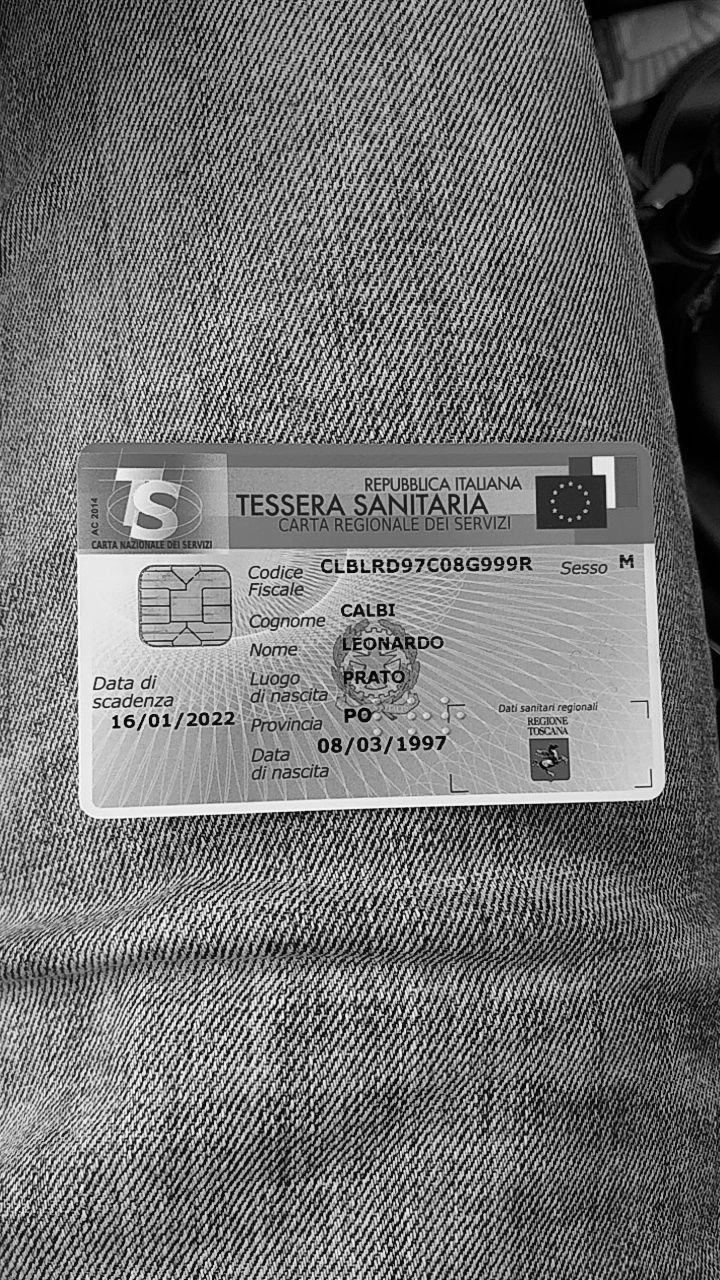
\includegraphics[width=.5\linewidth]{img/canny-hed-input.png}}
			}
		}
		\subfloat[][$\vars{thresh-low}=22$,\newline$\vars{thresh-high}=66$,\newline$\sigma=7$] {%
			\scalebox{0.5}[0.5] {
				\frame{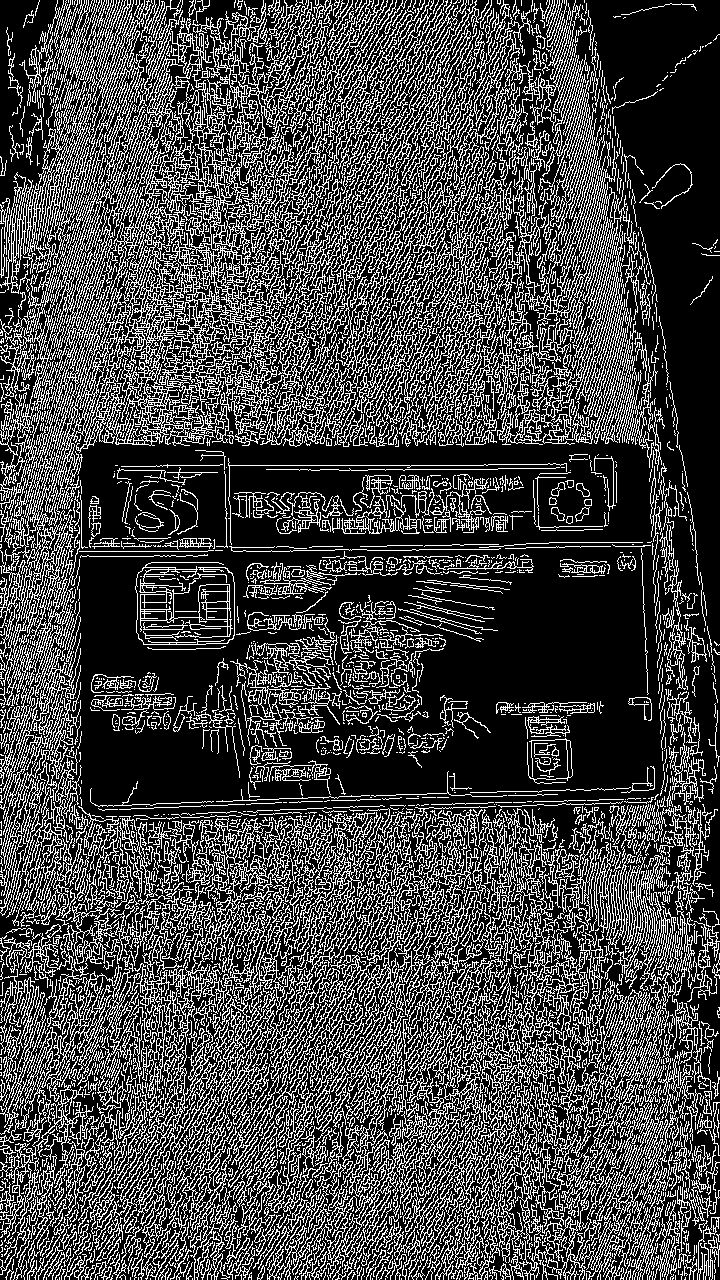
\includegraphics[width=.5\linewidth]{img/canny-min22-sigma7.png}}
			}
		}
		\subfloat[][$\vars{thresh-low}=55$,\newline$\vars{thresh-high}=165$,\newline$\sigma=6$] {%
			\scalebox{0.5}[0.5] {
				\frame{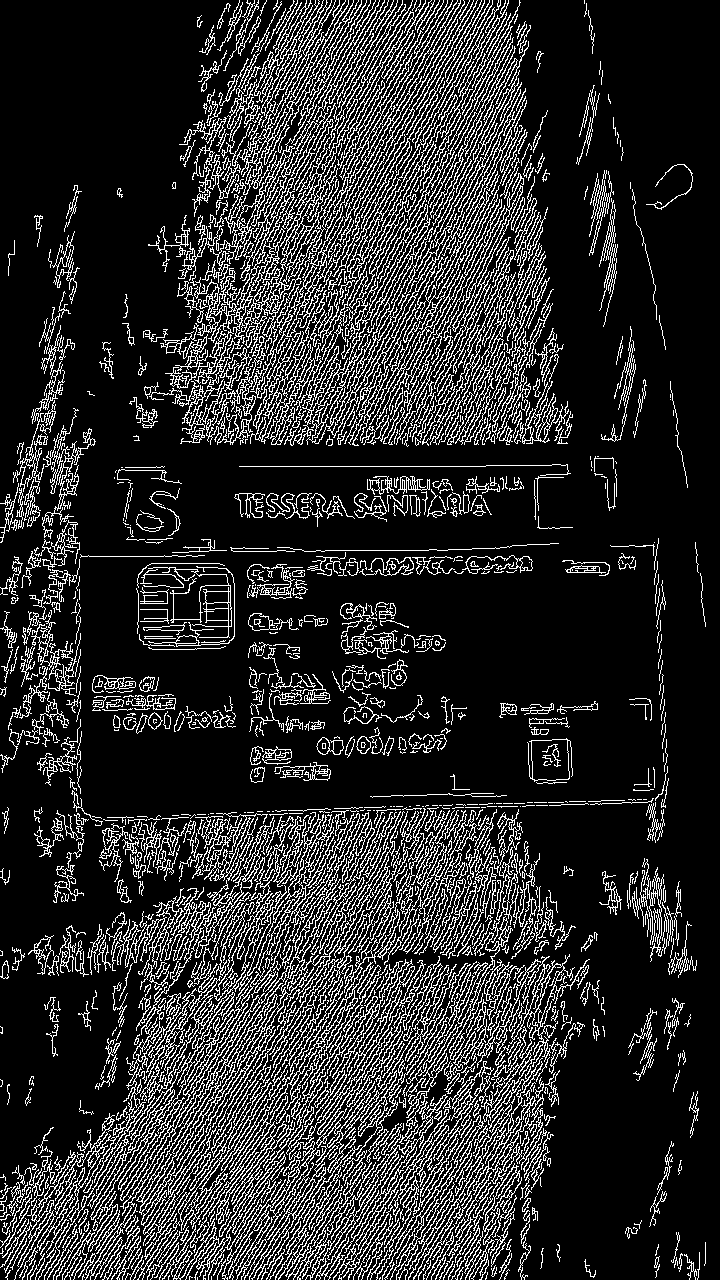
\includegraphics[width=.5\linewidth]{img/canny-min55-sigma6.png}}
			}
		}
		\subfloat[][$\vars{thresh-low}=100$,\newline$\vars{thresh-high}=255$,\newline$\sigma=2$] {%
			\scalebox{0.5}[0.5] {
				\frame{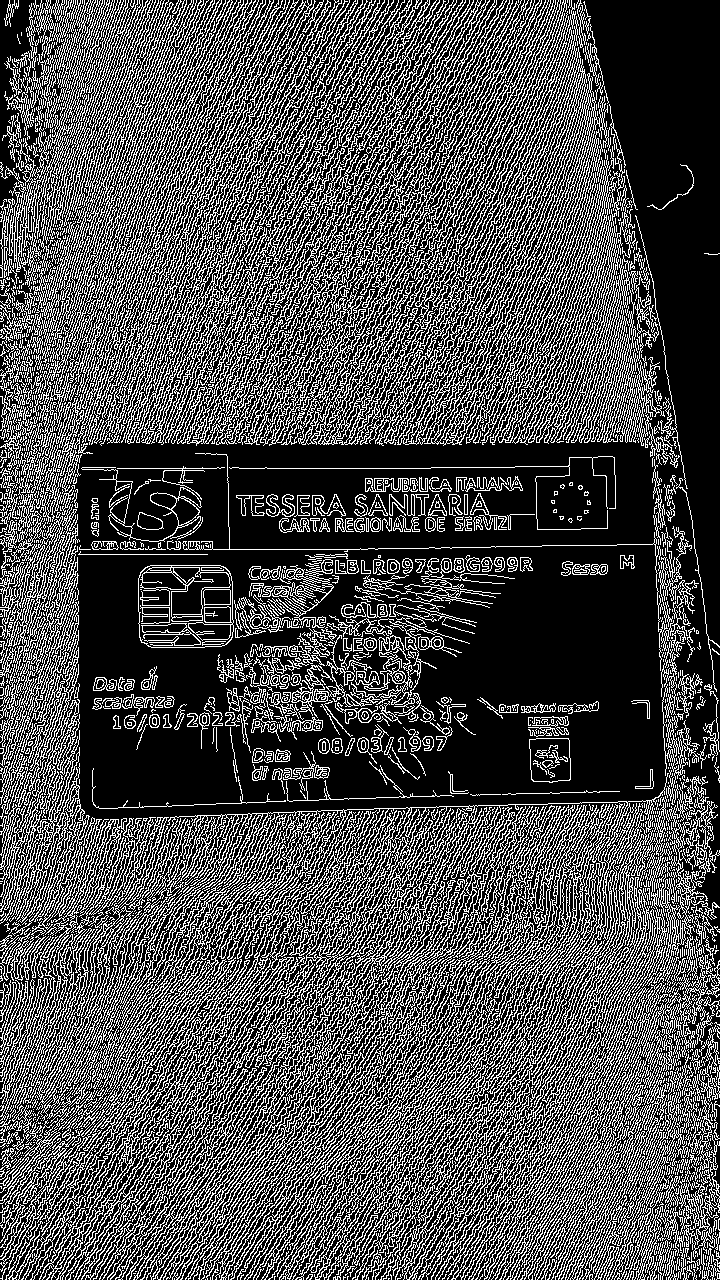
\includegraphics[width=.5\linewidth]{img/canny-min100-sigma2.png}}
			}
		}
	}
	\caption{Operatore \textit{Canny} con diversi parametri} \label{fig:canny}
\end{figure}

\subsection{HED}
L'approccio ideale per i problemi di \textit{edge detection} sarebbe quello di utilizzare un algoritmo che prende in input un'immagine e restituisce un'immagine binaria contenente informazioni sui bordi rilevanti dell'immagine in input, senza dover necessariamente impostare parametri diversi per contesti diversi.
\textit{HED} (\textit{Holistically-nested Edge Detection}) \cite{bib:hed} cerca di superare i limiti dell'operatore \textit{Canny}, tramite l'implementazione di una rete neurale convoluzionale. Le specifiche di questa soluzione non rientrano negli obiettivi di questa tesi, ma nelle figure \ref{fig:canny} e \ref{fig:hed} presentiamo un esempio di immagine processata sia dall'operatore \textit{Canny} che dalla rete \textit{HED}, per poter confrontare i risultati ottenuti.
\begin{figure}[h]
	\centering
	\resizebox{\textwidth}{!}{
		\centering
		\subfloat[Input] {%
			\scalebox{0.5}[0.5] {
				\frame{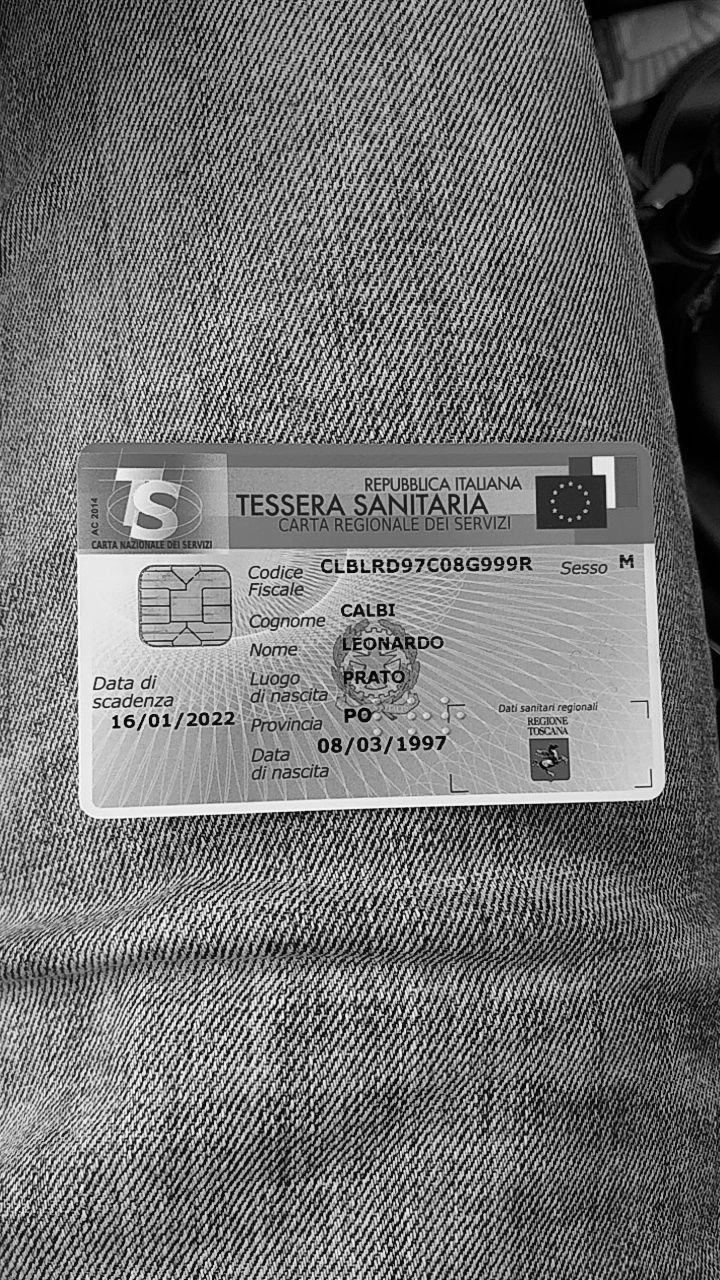
\includegraphics[width=.5\linewidth]{img/canny-hed-input.png}}
			}
		}
		\subfloat[Output] {%
			\scalebox{0.5}[0.5] {
				\frame{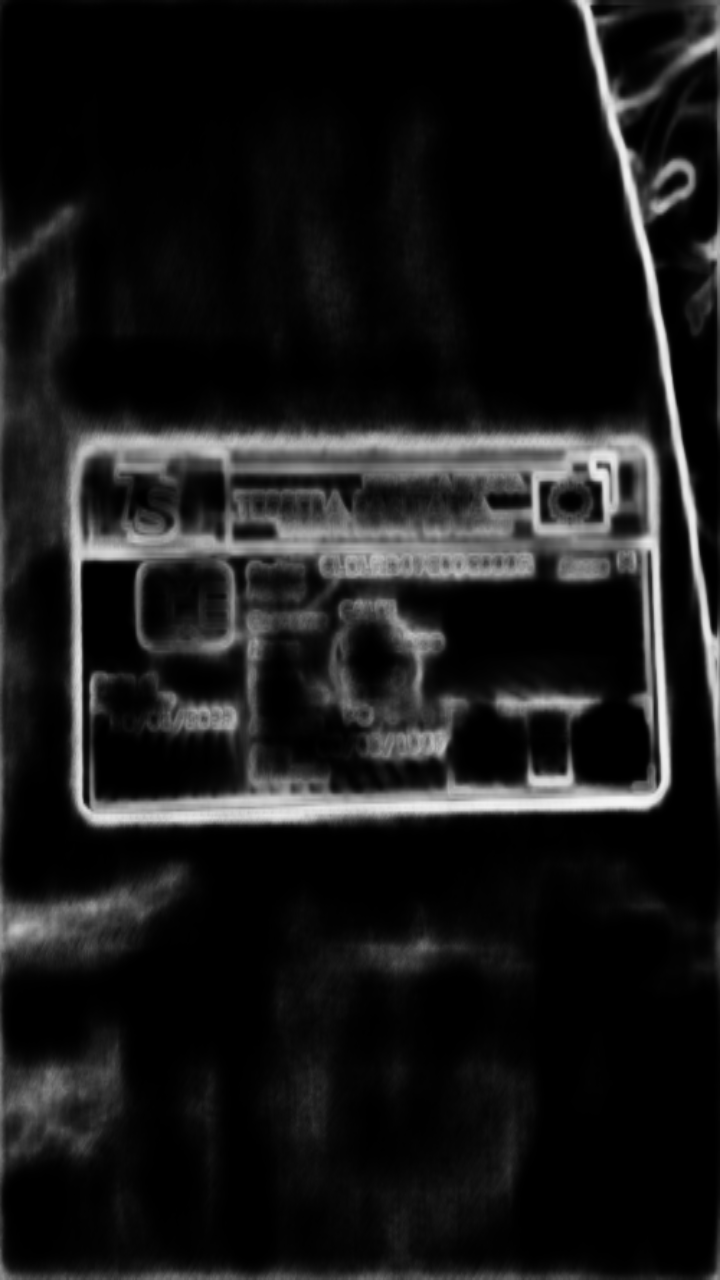
\includegraphics[width=.5\linewidth]{img/hed-output.png}}
			}
		}
		\subfloat[][Output con \textit{dilatazione}] {%
			\scalebox{0.5}[0.5] {
				\frame{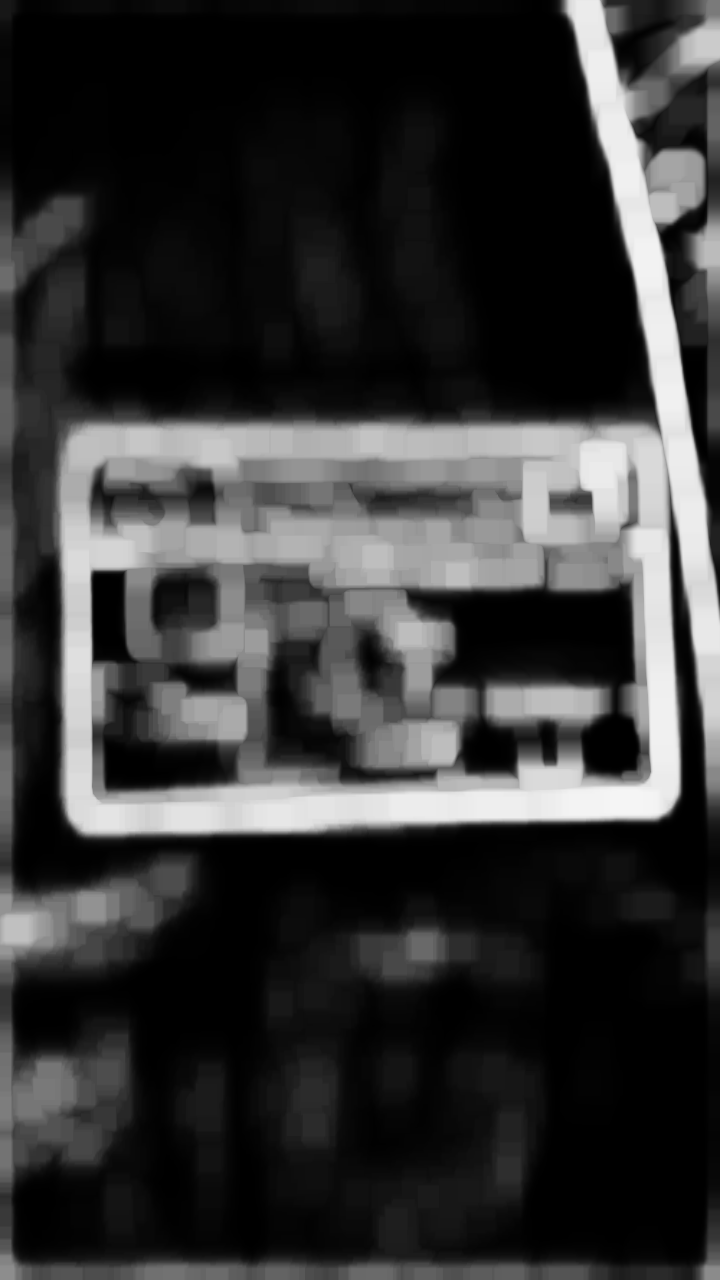
\includegraphics[width=.5\linewidth]{img/hed-output-dilated.png}}
			}
		}
	}
	\caption{Rete \textit{HED}} \label{fig:hed}
\end{figure}

\section{Implementazione}

\chapter{Text detection}
\label{chap:text-detection}


\section{Introduzione}
Negli ultimi anni, con l'avvento delle tecnologie di intelligenza artificiale e machine learning, gli algoritmi di rilevamento e riconoscimento del testo (\textit{text detection and recognition}) hanno subito un'evoluzione radicale, sia dal punto di vista dell'accuratezza dei risultati che dal punto di vista del tempo di esecuzione. Per quanto riguarda la \textit{text recognition} basta osservare il salto di qualit\`a subito da motori OCR open-source, quali \textit{Tesseract}, a seguito dell'implementazione di reti neurali ricorrenti (\textit{RNN}) di tipo \textit{LSTM} (\textit{Long Short Term Memory}), particolarmente adatte per questo tipo di applicazioni.\par
In questo capitolo ci concentriamo sull'introduzione di alcuni algoritmi di \textit{text detection}, che vengono utilizzati per riconoscere regioni di testo presenti in un'immagine e presentiamo un integrazione efficiente di questi metodi all'interno della libreria QI-OCR. 


\section{MSER}
Il metodo presentato in \cite{bib:mser} \`e un algoritmo di \textit{blob\footnote{Un blob in un'immagine \`e un gruppo connesso di pixel che condividono una determinata propriet\`a.} detection}, per la rilevazione di alcuni regioni distinguibili (\textit{DRs - Distinguished Regions}) in un'immagine, ovvero regioni che posseggono propriet\`a di stabilit\`a e invarianza, con un conseguente alto grado di ripetibilit\`a nella rilevazione.\par
Introduciamo delle regioni che vengono denominate \textit{ER (Extremal Regions)}, nel senso che tutti i pixel interni hanno intensit\`a esclusivamente maggiore o minore dei pixel nel contorno esterno della regione. Le \textit{ER} godono di due importanti propriet\`a: sono invarianti per trasformazioni geometriche affini e per trasformazioni monot\`one di intensit\`a dell'immagine. Le regioni di interesse sono un sottoinsieme delle \textit{ER} e vengono denominate \textit{MSER} (\textit{Maximally Stable Extremal Regions}), poich\`e risultano \textit{stabili} sotto una serie di operazioni di \textit{thresholding} e permettono una rilevazione multi-scala delle regioni, nel senso che vengono individuate sia strutture molto piccole che molto grandi.\par
Il grande vantaggio di questo \textit{blob detector} \`e la sua efficienza, in quanto l'enumerazione di tutte le \textit{ER} ha una complessit\`a temporale quasi lineare\footnote{In \cite{bib:mser-linear} \textit{Nist\'er} e \textit{Stew\'enius} propongono un metodo per l'enumerazione delle \textit{MSER} in tempo $\mathcal{O}(n)$, lineare nel numero di pixel dell'immagine.} di $\mathcal{O}(n\log{}\log{}n)$, data principalmente dall'algoritmo di enumerazione delle componenti connesse\footnote{Esiste una versione pi\`u efficiente, ma pi\`u articolata, dell'algoritmo per il \textit{labeling} delle componenti connesse (\textit{Rosenfeld-Pfaltz} \cite{bib:connected-components-fast}) con complessit\`a $\mathcal{O}(n\alpha(n))$, con $\alpha$ inversa della funzione di \textit{Ackermann}.}, con $n$ numero di pixel dell'immagine.\par
Nella pratica, l'algoritmo presentato pu\`o essere adattato per vari scopi e in particolare per il riconoscimento di testo in ambienti naturali, come descritto in \cite{bib:mser-canny}.\par
In figura \ref{fig:mser} un esempio di \textit{text detection} con l'utilizzo dell'algoritmo \textit{MSER} implementato nella libreria \textit{OpenCV}:
\begin{figure}[h]
	\centering
	\resizebox{\textwidth}{!}{
		\centering
		\subfloat[Input] {%
			\scalebox{0.5}[0.5] {
				\frame{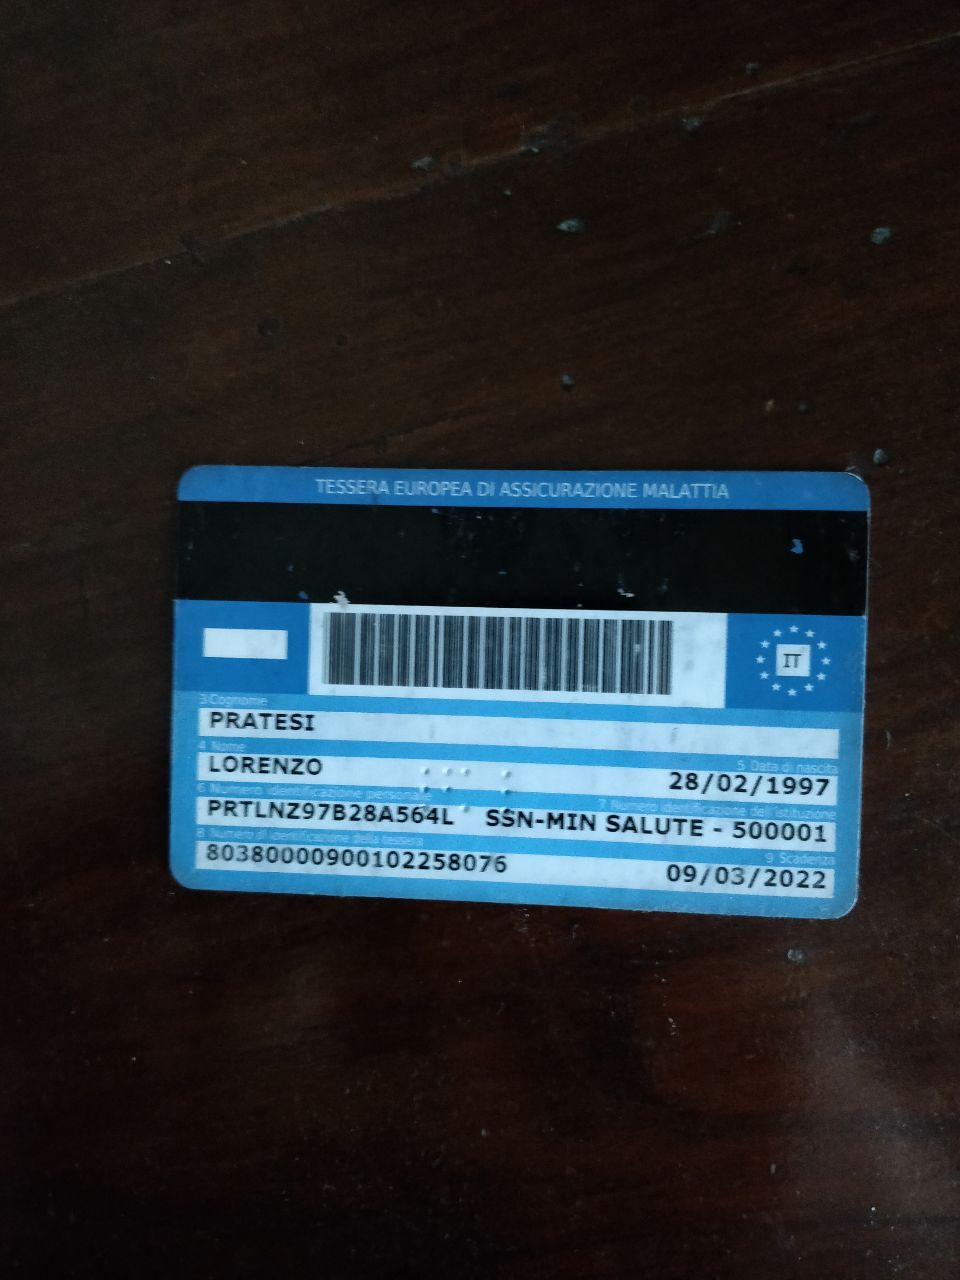
\includegraphics[width=.5\linewidth]{img/mser-east-input.png}}
			}
		}
		\subfloat[Output] {%
			\scalebox{0.5}[0.5] {
				\frame{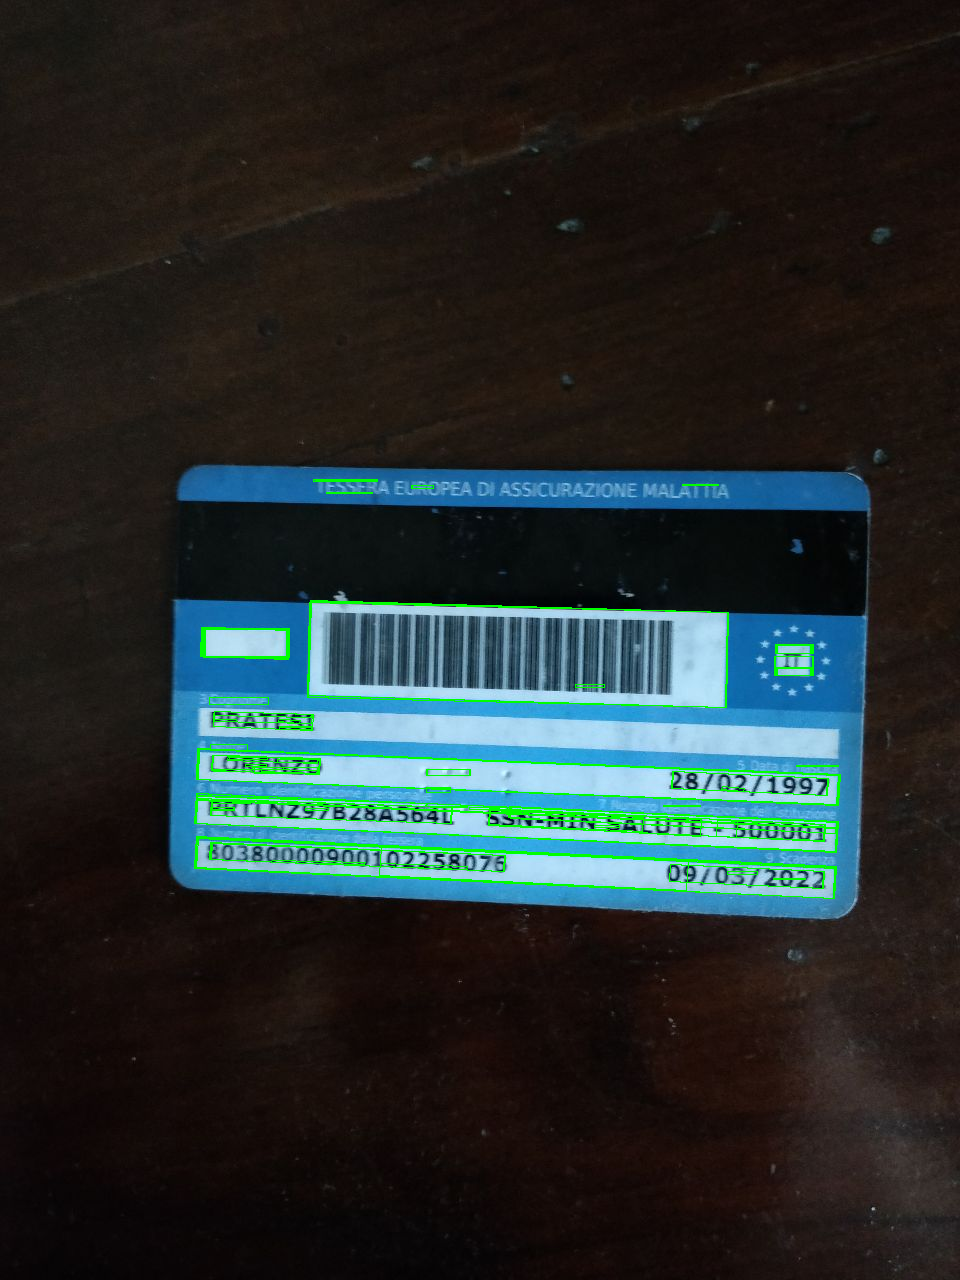
\includegraphics[width=.5\linewidth]{img/mser-regions.png}}
			}
		}
		\subfloat[][Output filtrato] {%
			\scalebox{0.5}[0.5] {
				\frame{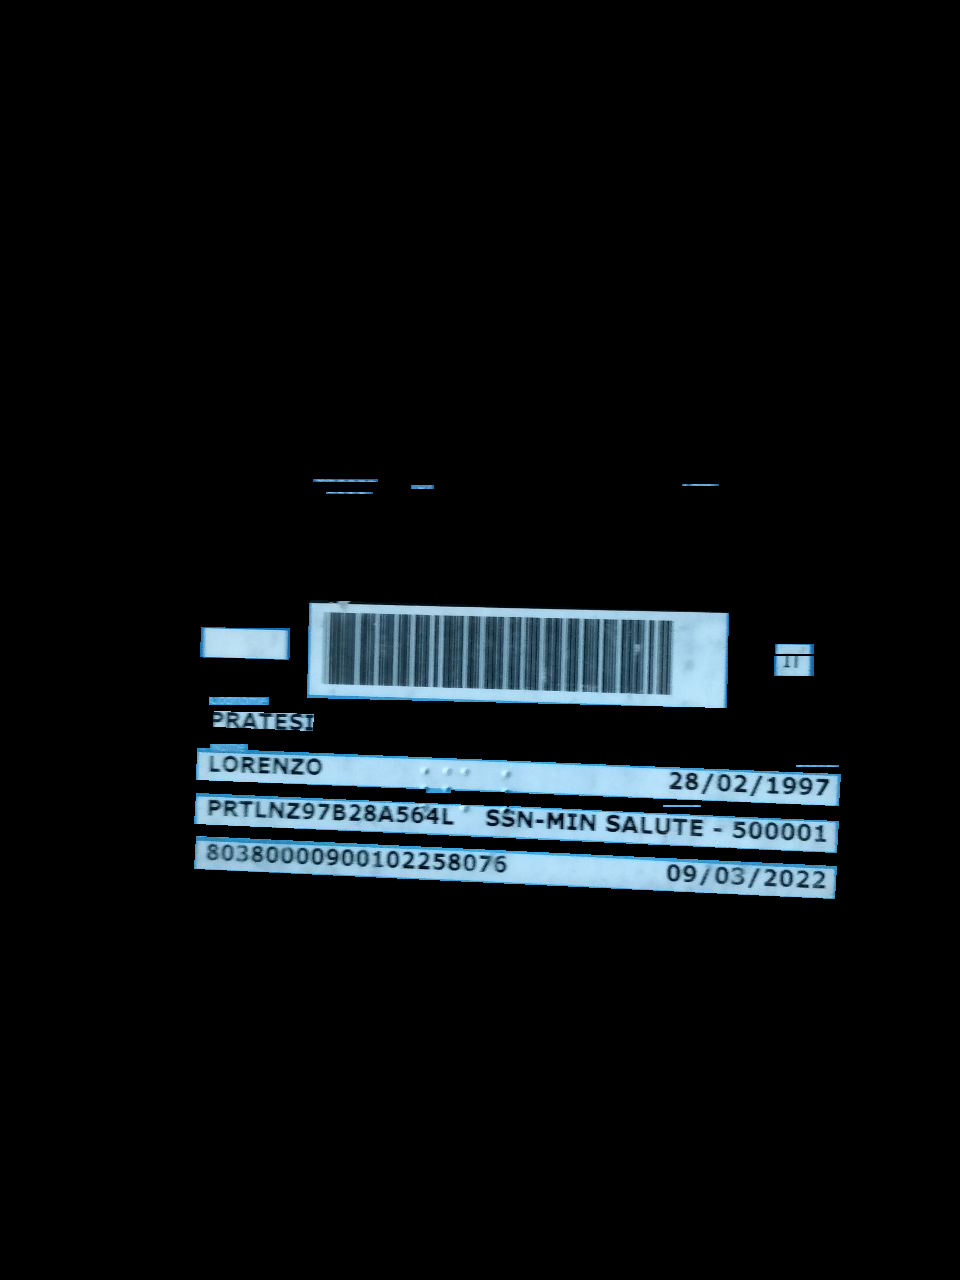
\includegraphics[width=.5\linewidth]{img/mser-regions-filtered.png}}
			}
		}
	}
	\caption{\textit{Text detection} con \textit{MSER}} \label{fig:mser}
\end{figure}


\section{EAST}
L'approccio ideale per i problemi di \textit{text detection} sarebbe quello di utilizzare un algoritmo che prende in input un'immagine e restituisce una lista di rettangoli, in cui ciascun rettangolo identifica una regione di testo dell'immagine. In base al tipo di \textit{text detection} che si intende effettuare, non orientata o orientata, ciascun rettangolo \`e identificato, rispettivamente, da una coppia $(x, y)$, $lunghezza$ e $altezza$, oppure da 4 coppie $(x, y)$ per ciascun vertice del rettangolo. Osservando l'output prodotto da \textit{MSER} in figura \ref{fig:mser}, \`e possibile constatare che le regioni restituite non sono solamente quelle contenenti testo. Infatti, nell'esempio riportato, viene evidenziata anche la regione contenente il \textit{codice a barre} del documento.\par 
\textit{EAST} (\textit{Efficient and Accurate Scene Text detector}) \cite{bib:east} cerca di superare i limiti di \textit{blob detector} come \textit{MSER}, tramite l'implementazione di una rete neurale convoluzionale (\textit{FCN - Fully Convolutional Network}). Le specifiche di questa soluzione non rientrano negli obiettivi di questa tesi, ma nelle figure \ref{fig:mser} e \ref{fig:east} presentiamo un esempio di immagine processata sia da \textit{MSER} che dalla rete \textit{EAST}, per poter confrontare i risultati ottenuti.
\begin{figure}[h]
	\centering
	\resizebox{\textwidth}{!}{
		\centering
		\subfloat[Input] {%
			\scalebox{0.5}[0.5] {
				\frame{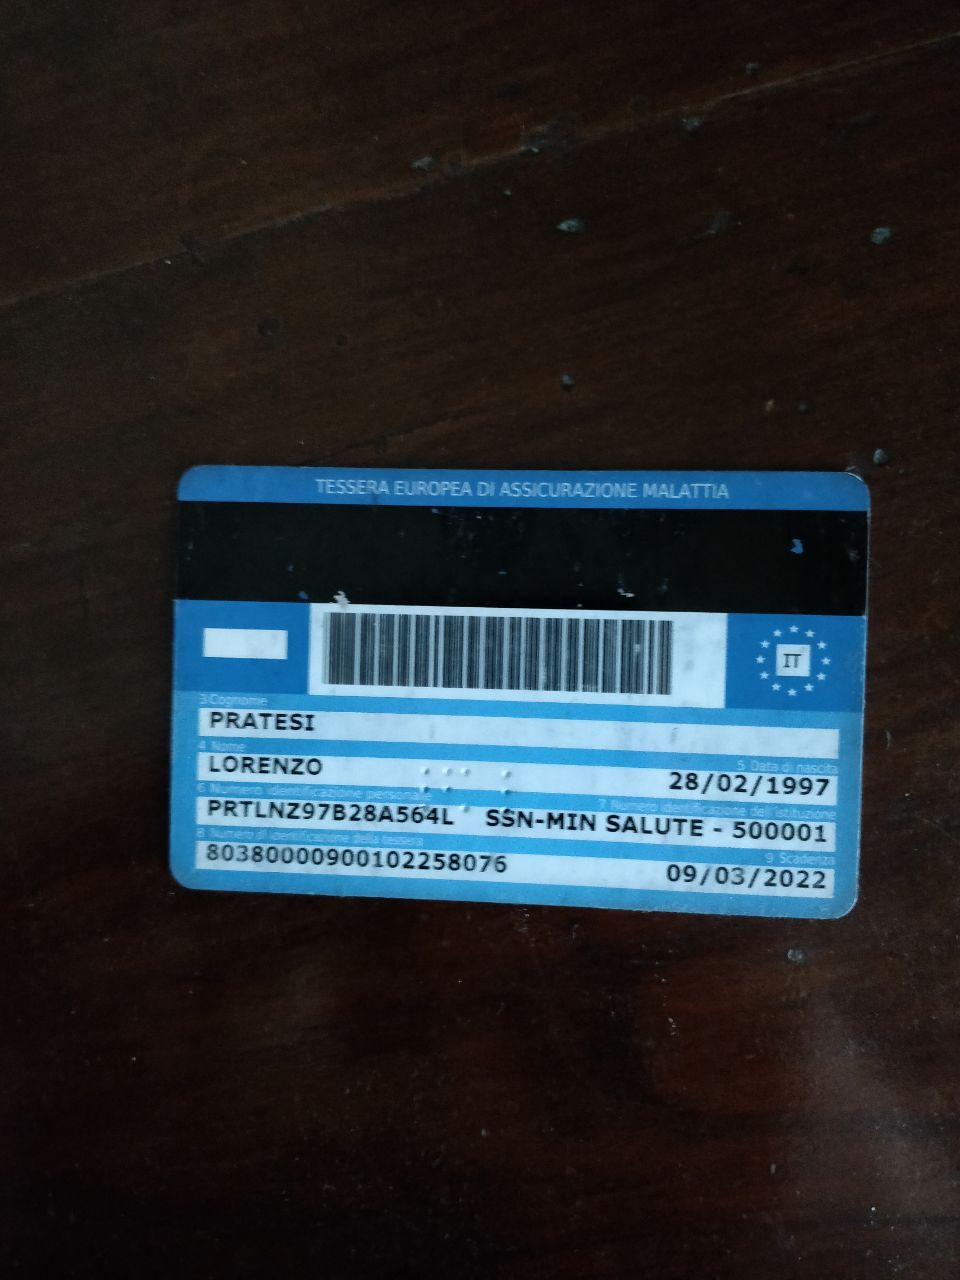
\includegraphics[width=.8\linewidth]{img/mser-east-input.png}}
			}
		}
		\subfloat[Output] {%
			\scalebox{0.5}[0.5] {
				\frame{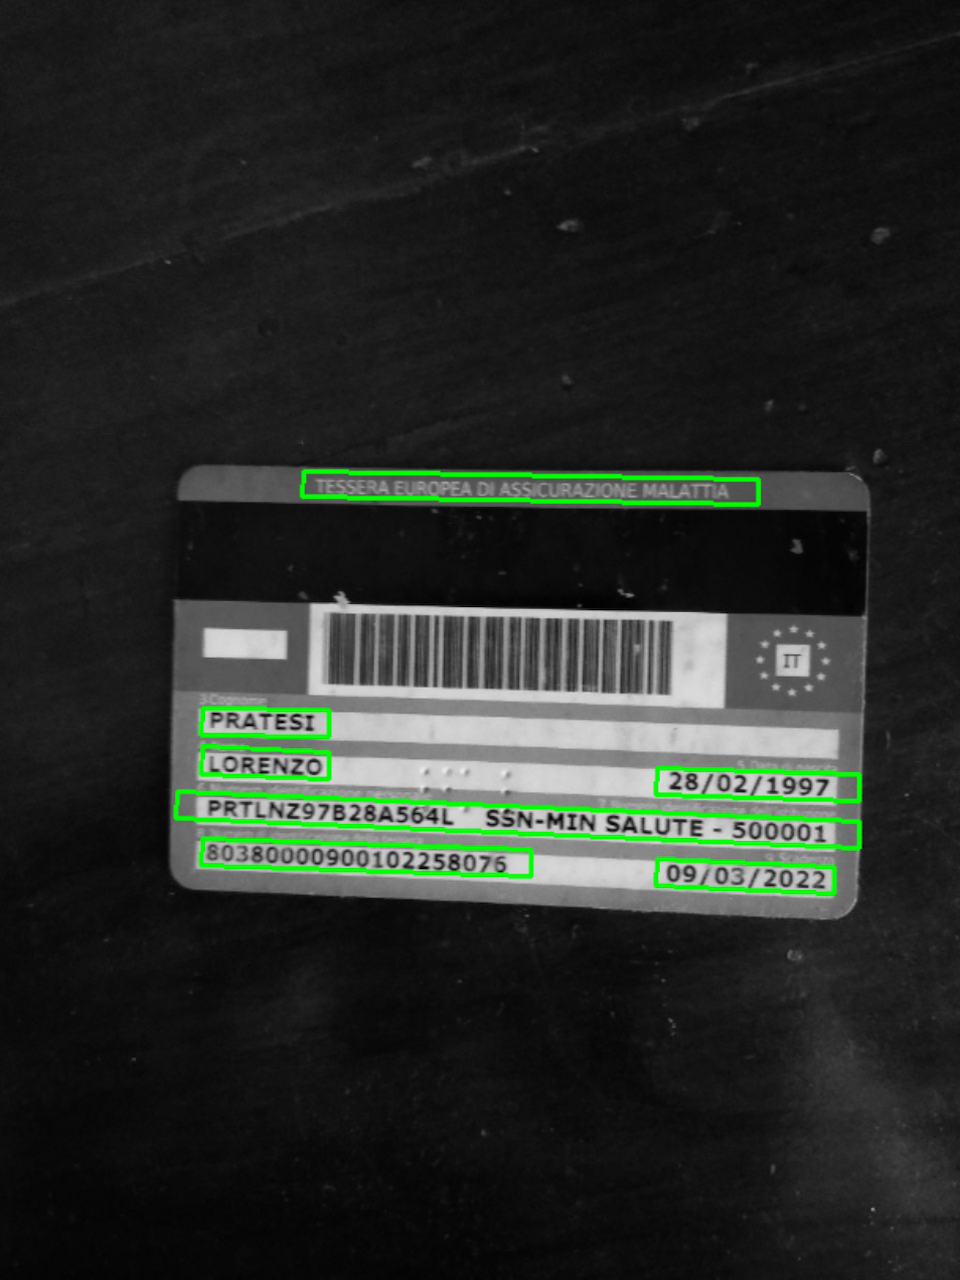
\includegraphics[width=.79\linewidth]{img/east-output.png}}
			}
		}
	}
	\caption{\textit{Text detection} con \textit{EAST}} \label{fig:east}
\end{figure}


\section{Ritaglio dinamico dei campi di un documento}
In questa sezione presentiamo un approccio dinamico per il ritaglio dei campi di un documento d'identit\`a. Prima dell'introduzione di questo metodo, la libreria QI-OCR effettuava un ritaglio statico per ogni campo del documento in analisi, in base a coordinate predeterminate dal \textit{template} del documento e ipotizzando un ritaglio e una centratura quasi perfetta a seguito degli algoritmi di localizzazione descritti nel capitolo \ref{chap:image-matching}. In tabella \ref{tab:car-r-coords} un esempio di coordinate definite per il retro della vecchia carta d'identit\`a italiana, in base a una dimensione di $700 \times 1000$ pixel, con campi e template visibili in figura \ref{fig:car-r-template}.\par
\begin{figure}[h]
	\centering
	\resizebox{.6\textwidth}{!}{
		\centering
		\subfloat[Template] {%
			\scalebox{0.5}[0.5] {
				\frame{
\includegraphics[width=.5\linewidth]{img/car-r-template.png}}
			}
		}
		\subfloat[Campi] {%
			\scalebox{0.5}[0.5] {
				\frame{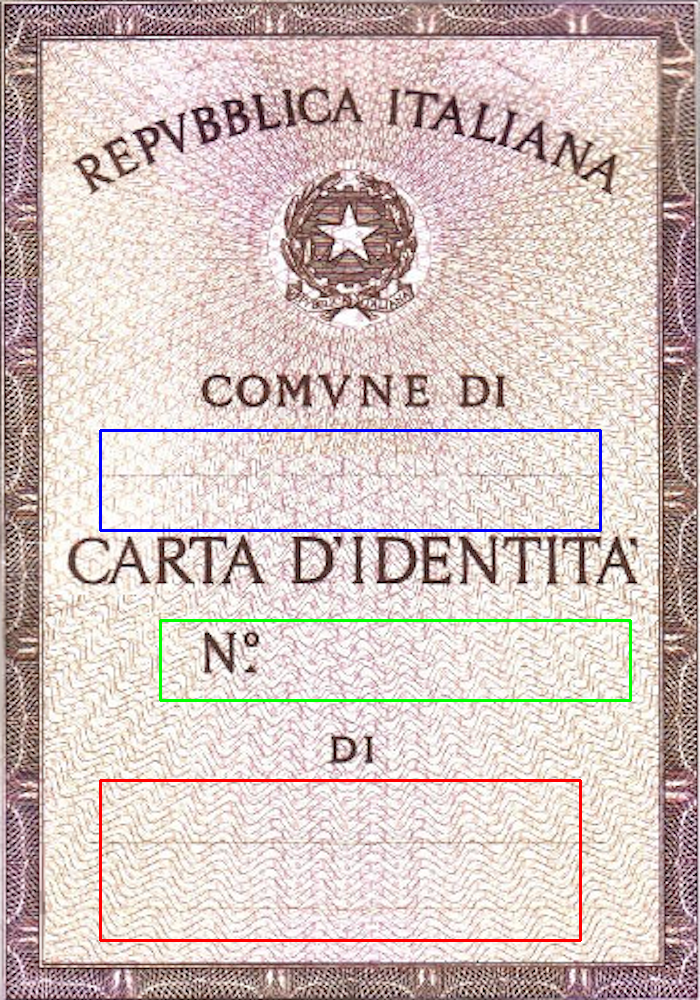
\includegraphics[width=.5\linewidth]{img/car-r-fields.png}}
			}
		}
	}
	\caption{Campi vecchia carta d'identit\`a italiana (retro)} \label{fig:car-r-template}
\end{figure}
\begin{table}[H]
	\centering
	\resizebox{.8\textwidth}{!}{%
	\begin{tabular}{|c|c|c|c|c|}
	\hline
	\textbf{Campo} & \textbf{$x$} & \textbf{$y$} & \textbf{$larghezza$} & \textbf{$altezza$} \\ \hline
	{\color{blue}Comune} & $100px$ & $430px$ & $500px$ & $100px$ \\ \hline
	{\color{green}Numero documento} & $160px$ & $620px$ & $470px$ & $80px$ \\ \hline
	{\color{red}Nome completo} & $100px$ & $780px$ & $480px$ & $160px$ \\ \hline
	\end{tabular}%
	}
	\caption{Coordinate campi vecchia carta d'identit\`a italiana (retro)}
	\label{tab:car-r-coords}
\end{table}
Purtroppo, con il ritaglio statico utilizzato il rischio di perdita d'informazione aumenta quando la localizzazione del documento ritorna un risultato approssimativo, oppure quando si stanno estraendo campi da documenti che non rispettano esattamente i template prefissati, come la vecchia carta d'identit\`a italiana. Per avere un'idea pi\`u concreta della problematica menzionata, in figura \ref{fig:car-f-example} mostriamo un esempio di carta d'identit\`a cartacea che non rispetta gli standard e in figura \ref{fig:car-f-static} i relativi campi ritagliati in modo statico.\par
\begin{figure}[H]
	\centering
	\resizebox{.5\textwidth}{!}{
		\frame{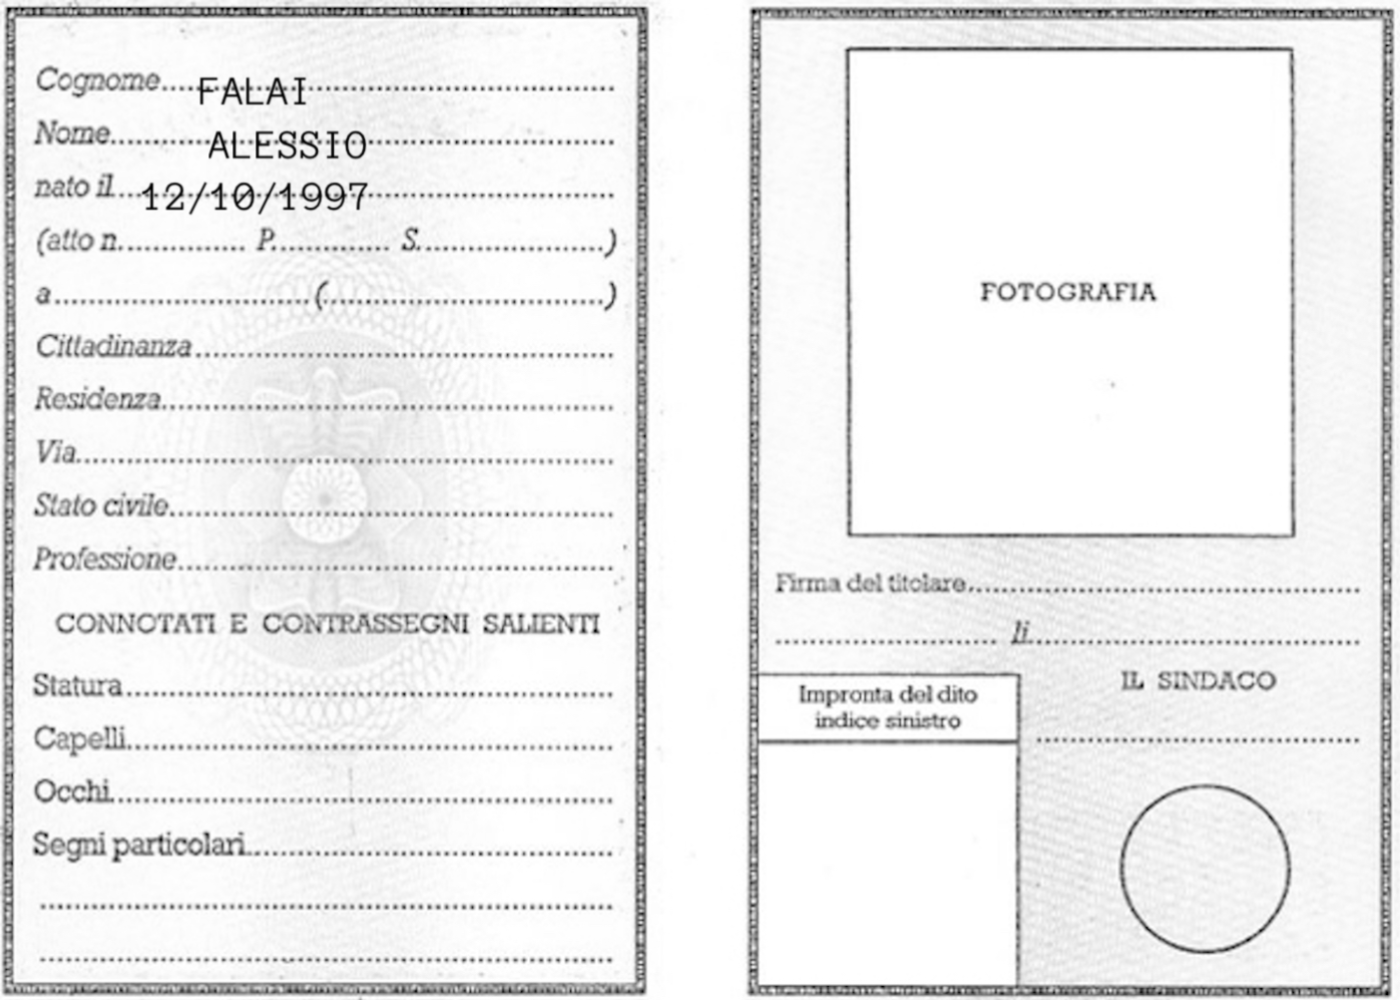
\includegraphics[]{img/car-f.png}}
	}
	\caption{Vecchia carta d'identit\`a italiana (fronte) non standard} \label{fig:car-f-example}
\end{figure}
\begin{figure}[h]
	\centering
	\resizebox{\textwidth}{!}{
		\centering
		\subfloat[Nome] {%
			\scalebox{0.5}[0.5] {
				\frame{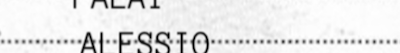
\includegraphics[width=.5\linewidth]{img/car-f-name-static.png}}
			}
		}
		\subfloat[Cognome] {%
			\scalebox{0.5}[0.5] {
				\frame{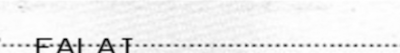
\includegraphics[width=.5\linewidth]{img/car-f-surname-static.png}}
			}
		}
		\subfloat[Data di nascita] {%
			\scalebox{0.5}[0.5] {
				\frame{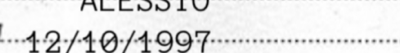
\includegraphics[width=.5\linewidth]{img/car-f-birthdate-static.png}}
			}
		}
	}
	\caption{Campi vecchia carta d'identit\`a italiana (fronte) non standard, ritagliati in modo statico} \label{fig:car-f-static}
\end{figure}
L'approccio proposto consente di risolvere le problematiche del ritaglio statico, quando lo scostamento delle coordinate reali da quelle predefinite non \`e troppo elevato. L'algoritmo in questione prevede l'individuazione delle regioni di testo in modo dinamico, tramite uno degli algoritmi di \textit{text detection} descritti. Dopodich\`e, per ciascun campo, le informazioni sui \textit{bounding boxes dinamici} vengono utilizzate per calcolare il valore di ordinata effettivo e la lunghezza corretta del campo in esame. Per svolgere questo compito, l'algoritmo computa l'intersezione del rettangolo statico con tutti i rettangoli dinamici e calcola l'area di intersezione massima. Le coordinate del \textit{bounding box dinamico} che ha dato l'intersezione di area massima vengono utilizzate per determinare i nuovi valori di $y$ e $lunghezza$ del campo analizzato. Lo pseudocodice della procedura descritta \`e definito nell'algoritmo \ref{alg:dynamic-cut}, mentre l'immagine \ref{fig:car-f-dynamic} mostra i risultati ottenuti nell'esempio riportato in figura \ref{fig:car-f-example}, grazie all'utilizzo della rete \textit{EAST} (vedi figura \ref{fig:car-f-example-east}).
\begin{figure}[H]
	\centering
	\resizebox{.5\textwidth}{!}{
		\frame{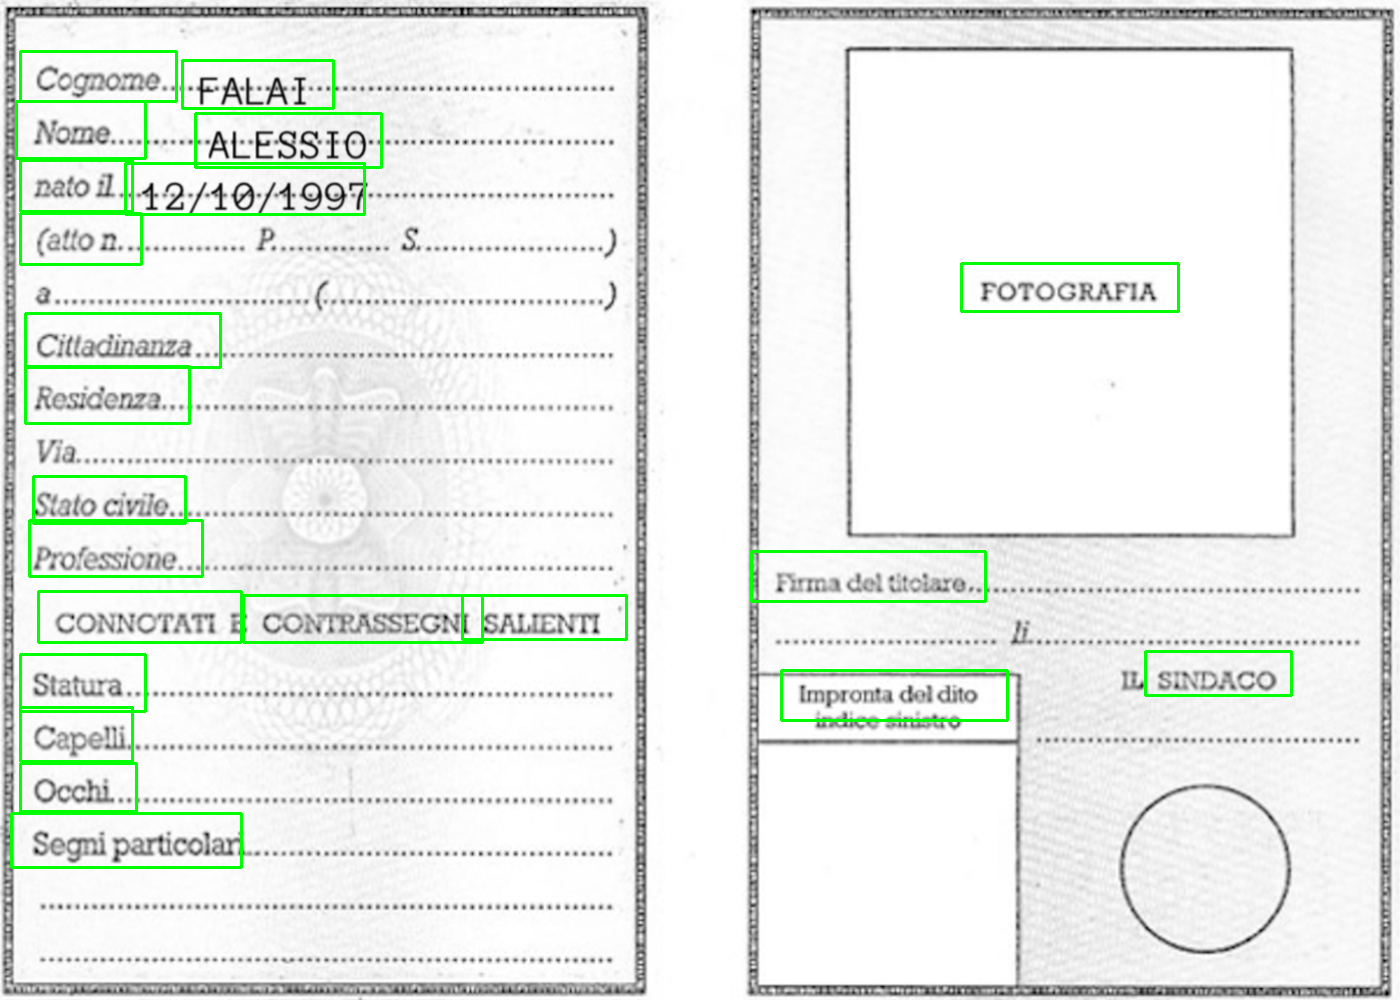
\includegraphics[]{img/car-f-east.png}}
	}
	\caption{Output di \textit{EAST} su una vecchia carta d'identit\`a italiana (fronte) non standard} \label{fig:car-f-example-east}
\end{figure}
\begin{figure}[H]
	\centering
	\resizebox{\textwidth}{!}{
		\centering
		\subfloat[Nome] {%
			\scalebox{0.5}[0.5] {
				\frame{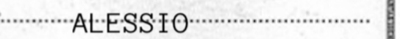
\includegraphics[width=.5\linewidth]{img/car-f-name-dynamic.png}}
			}
		}
		\subfloat[Cognome] {%
			\scalebox{0.5}[0.5] {
				\frame{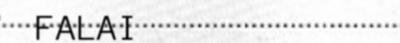
\includegraphics[width=.5\linewidth]{img/car-f-surname-dynamic.png}}
			}
		}
		\subfloat[Data di nascita] {%
			\scalebox{0.5}[0.5] {
				\frame{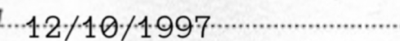
\includegraphics[width=.5\linewidth]{img/car-f-birthdate-dynamic.png}}
			}
		}
	}
	\caption{Campi vecchia carta d'identit\`a italiana (fronte) non standard, ritagliati in modo dinamico} \label{fig:car-f-dynamic}
\end{figure}

\begin{algorithm}[H]
	\caption{Ritaglio dinamico}
	\label{alg:dynamic-cut}
	
	\begin{algorithmic}[1]
		\Function{dynamic-cut}{}
			\State $\vars{image} \gets \text{input image}$
			\State $\vars{field} \gets \text{rectangle} (\vars{x}, \vars{y}, \vars{width}, \vars{height})$
			\State $\vars{dynamic-fields} \gets \text{list of rectangles} (\vars{x}, \vars{y}, \vars{width}, \vars{height})$
			\\
			\State $\vars{max-bbox} \gets \textproc{max-intersection-area-bbox(\vars{field}, \vars{dynamic-fields})}$
			\State $\vars{field.y} \gets \vars{max-bbox.y}$
			\State $\vars{field.width} \gets \textproc{max(\vars{field.width, max-bbox.width})}$

			\Return $\vars{image[field.y:field.y + field.height]}$\newline\hspace*{2.91cm}
					$\vars{[field.x:field.x + field.width]}$
		\EndFunction
		\Statex
		\Function{max-intersection-area-bbox}{}
			\State $\vars{field} \gets \text{rectangle} (\vars{x}, \vars{y}, \vars{width}, \vars{height})$
			\State $\vars{dynamic-fields} \gets \text{list of rectangles} (\vars{x}, \vars{y}, \vars{width}, \vars{height})$
			\\
			\State $\vars{max-area} \gets 0\text{, } \vars{max-bbox} \gets field$
			\For {$\vars{dynamic-field} \text{ in \vars{dynamic-fields}}$}
				\State $\vars{area} \gets \textproc{intersection-area(\vars{field}, \vars{dynamic-field})}$
				\If {$\vars{area} > \vars{max-area}$}
					\State $\vars{max-area} \gets \vars{area}$
					\State $\vars{max-bbox} \gets \vars{dynamic-field}$
				\EndIf
			\EndFor

			\Return $\vars{max-bbox}$
		\EndFunction
	\end{algorithmic}
\end{algorithm}

\chapter*{Conclusioni e sviluppi futuri}
\addcontentsline{toc}{chapter}{Conclusioni e sviluppi futuri}

\chapter*{Ringraziamenti}
\addcontentsline{toc}{chapter}{Ringraziamenti}
\markboth{Ringraziamenti}{Ringraziamenti}

Innanzitutto desidero ringraziare la mia famiglia. Ringrazio i miei genitori e i miei nonni per avermi sempre sostenuto, in ogni mia scelta. Allo stesso modo ringrazio mio fratello per essere sempre stato un punto di riferimento.\par
Ringrazio Silvia per essere sempre stata al mio fianco e per avermi aiutato ad affrontare col sorriso qualunque difficolt\`a.\par
Ringrazio i miei compagni di studi e in particolare Leonardo, Jacopo e Lorenzo, con i quali ho avuto il piacere di condividere questa esperienza.\par
Ringrazio i miei amici e in particolare Saul, che per me c'\`e sempre stato.\par
Infine ringrazio Michele Barbagli, per aver reso possibile la collaborazione che mi ha permesso di scrivere questa tesi e arricchire le mie conoscenze professionali.

\addcontentsline{toc}{chapter}{Bibliografia}
\markboth{Bibliografia}{Bibliografia}
\begin{thebibliography}{99}

\bibitem{bib:digital-image-processing}{Wilhelm Burger, Mark J. Burge - \emph{Digital Image Processing - An Algorithmic Introduction Using Java, Second Edition}}

\bibitem{bib:convolution}{Raffaele Cappelli - \emph{Fondamenti di Elaborazione di Immagini - Operazioni sulle immagini} - Universit\`a degli Studi di Bologna}

\bibitem{bib:wikipedia}{Wikipedia - \emph{\url{https://it.wikipedia.org}}}

\bibitem{bib:top-hat-paper}{Guocheng Wang, Yiwen Wang, Hui Li, Xuanqi Chen, Haitao Lu,
Yanpeng Ma, Chun Peng, Yijun Wang, Linyao Tang - \emph{Morphological Background Detection and Illumination Normalization of Text Image with Poor Lighting} - PLOS ONE}

\bibitem{bib:opencv}{OpenCV documentation - \emph{\url{https://docs.opencv.org}}}

\bibitem{bib:skin-thesis}{Simone Parca - \emph{Studio e sviluppo di algoritmi per l'analisi di immagini della pelle acquisite tramite un sensore capacitivo} - Universit\`a degli Studi di Bologna}

\bibitem{bib:binary-images-connectivity}{Francesco Tortorella - \emph{Elementi di geometria delle immagini digitali binarie} - Universit\`a degli studi di Cassino e del Lazio Meridionale}

\bibitem{bib:advanced-morphological}{\emph{Advanced morphological image processing} - University of Groningen}

\bibitem{bib:niblack}{W. Niblack - \emph{An introduction to Digital Image Processing} - Prentice-Hall}

\bibitem{bib:sauvola}{J. Sauvola, M. Pietikainen - \emph{Adaptive document image binarization} - Pattern Recognition 33(2), pp. 225-236}

\bibitem{bib:medium-feature-matching}{Deepanshu Tyagi - \emph{Introduction To Feature Detection And Matching} - \url{https://medium.com}}

\bibitem{bib:text-extraction}{P. Nagabhushan, S. Nirmala - \emph{Text Extraction in Complex Color Document Images for Enhanced Readability}}

\bibitem{bib:sift}{David G. Lowe - \emph{Distinctive Image Features from Scale-Invariant Keypoints} - University of British Columbia}

\bibitem{bib:surf}{Herbert Bay, Tinne Tuytelaars, Luc Van Gool - \emph{SURF: Speeded Up Robust Features}}

\bibitem{bib:kaze}{Pablo Fern\`andez Alcantarilla, Adrien Bartoli, Andrew J. Davison - \emph{KAZE Features}}

\bibitem{bib:akaze}{Pablo F. Alcantarilla, Jes\`us Nuevo, Adrien Bartoli - \emph{Fast Explicit Diffusion for Accelerated Features in Nonlinear Scale Spaces}}

\bibitem{bib:brisk}{Stefan Leutenegger, Margarita Chli, Roland Y. Siegwart - \emph{BRISK: Binary Robust Invariant Scalable Keypoints}}

\bibitem{bib:orb}{Ethan Rublee, Vincent Rabaud, Kurt Konolige, Gary Bradski - \emph{ORB: an efficient alternative to SIFT or SURF}}

\bibitem{bib:prewitt}{J. Prewitt - \emph{Object enhancement and extraction} - Picture Processing and Psychopictorics, pp. 415-431}

\bibitem{bib:canny}{John Canny - \emph{A Computational Approach to Edge Detection}}

\bibitem{bib:hed}{Saining Xie, Zhuowen Tu - \emph{Holistically-Nested Edge Detection}}

\bibitem{bib:mser}{J. Matas, O. Chum, M. Urban, T. Pajdla - \emph{Robust Wide Baseline Stereo from Maximally Stable Extremal Regions}}

\bibitem{bib:mser-linear}{David Nist\`er, Henrik Stew\`enius - \emph{Linear Time Maximally Stable Extremal Regions}}

\bibitem{bib:connected-components-fast}{Azriel Rosenfeld, John L. Pfaltz - \emph{Sequential Operations in Digital Picture Processing}}

\bibitem{bib:mser-canny}{Huizhong Chen, Sam S. Tsai, Georg Schroth, David M. Chen, Radek Grzeszczuk and Bernd Girod - \emph{Robust text detection in natural images with edge-enhanced Maximally Stable Extremal Regions}}

\bibitem{bib:east}{Xinyu Zhou, Cong Yao, He Wen, Yuzhi Wang, Shuchang Zhou, Weiran He, Jiajun Liang - \emph{EAST: An Efficient and Accurate Scene Text Detector}}

\end{thebibliography}

%--------------------------------------------------------------
\end{document}
%--------------------------------------------------------------
